\documentclass[twoside]{book}

% Packages required by doxygen
\usepackage{fixltx2e}
\usepackage{calc}
\usepackage{doxygen}
\usepackage[export]{adjustbox} % also loads graphicx
\usepackage{graphicx}
\usepackage[utf8]{inputenc}
\usepackage{makeidx}
\usepackage{multicol}
\usepackage{multirow}
\PassOptionsToPackage{warn}{textcomp}
\usepackage{textcomp}
\usepackage[nointegrals]{wasysym}
\usepackage[table]{xcolor}

% Font selection
\usepackage[T1]{fontenc}
\usepackage[scaled=.90]{helvet}
\usepackage{courier}
\usepackage{amssymb}
\usepackage{sectsty}
\renewcommand{\familydefault}{\sfdefault}
\allsectionsfont{%
  \fontseries{bc}\selectfont%
  \color{darkgray}%
}
\renewcommand{\DoxyLabelFont}{%
  \fontseries{bc}\selectfont%
  \color{darkgray}%
}
\newcommand{\+}{\discretionary{\mbox{\scriptsize$\hookleftarrow$}}{}{}}

% Page & text layout
\usepackage{geometry}
\geometry{%
  a4paper,%
  top=2.5cm,%
  bottom=2.5cm,%
  left=2.5cm,%
  right=2.5cm%
}
\tolerance=750
\hfuzz=15pt
\hbadness=750
\setlength{\emergencystretch}{15pt}
\setlength{\parindent}{0cm}
\setlength{\parskip}{3ex plus 2ex minus 2ex}
\makeatletter
\renewcommand{\paragraph}{%
  \@startsection{paragraph}{4}{0ex}{-1.0ex}{1.0ex}{%
    \normalfont\normalsize\bfseries\SS@parafont%
  }%
}
\renewcommand{\subparagraph}{%
  \@startsection{subparagraph}{5}{0ex}{-1.0ex}{1.0ex}{%
    \normalfont\normalsize\bfseries\SS@subparafont%
  }%
}
\makeatother

% Headers & footers
\usepackage{fancyhdr}
\pagestyle{fancyplain}
\fancyhead[LE]{\fancyplain{}{\bfseries\thepage}}
\fancyhead[CE]{\fancyplain{}{}}
\fancyhead[RE]{\fancyplain{}{\bfseries\leftmark}}
\fancyhead[LO]{\fancyplain{}{\bfseries\rightmark}}
\fancyhead[CO]{\fancyplain{}{}}
\fancyhead[RO]{\fancyplain{}{\bfseries\thepage}}
\fancyfoot[LE]{\fancyplain{}{}}
\fancyfoot[CE]{\fancyplain{}{}}
\fancyfoot[RE]{\fancyplain{}{\bfseries\scriptsize Generated by Doxygen }}
\fancyfoot[LO]{\fancyplain{}{\bfseries\scriptsize Generated by Doxygen }}
\fancyfoot[CO]{\fancyplain{}{}}
\fancyfoot[RO]{\fancyplain{}{}}
\renewcommand{\footrulewidth}{0.4pt}
\renewcommand{\chaptermark}[1]{%
  \markboth{#1}{}%
}
\renewcommand{\sectionmark}[1]{%
  \markright{\thesection\ #1}%
}

% Indices & bibliography
\usepackage{natbib}
\usepackage[titles]{tocloft}
\setcounter{tocdepth}{3}
\setcounter{secnumdepth}{5}
\makeindex

% Hyperlinks (required, but should be loaded last)
\usepackage{ifpdf}
\ifpdf
  \usepackage[pdftex,pagebackref=true]{hyperref}
\else
  \usepackage[ps2pdf,pagebackref=true]{hyperref}
\fi
\hypersetup{%
  colorlinks=true,%
  linkcolor=blue,%
  citecolor=blue,%
  unicode%
}

% Custom commands
\newcommand{\clearemptydoublepage}{%
  \newpage{\pagestyle{empty}\cleardoublepage}%
}

\usepackage{caption}
\captionsetup{labelsep=space,justification=centering,font={bf},singlelinecheck=off,skip=4pt,position=top}

%===== C O N T E N T S =====

\begin{document}

% Titlepage & ToC
\hypersetup{pageanchor=false,
             bookmarksnumbered=true,
             pdfencoding=unicode
            }
\pagenumbering{roman}
\begin{titlepage}
\vspace*{7cm}
\begin{center}%
{\Large S\+P\+MB }\\
\vspace*{1cm}
{\large Generated by Doxygen 1.8.11}\\
\end{center}
\end{titlepage}
\clearemptydoublepage
\tableofcontents
\clearemptydoublepage
\pagenumbering{arabic}
\hypersetup{pageanchor=true}

%--- Begin generated contents ---
\chapter{S\+P\+MB}
\label{index}\hypertarget{index}{}\subsection*{Brief}

The Signal\&Power Management Board ({\bfseries \hyperlink{namespaceSPMB}{S\+P\+MB}}) provides firmware for Arduino U\+NO devices using Atmega328p microcontrollers facilitating a Robot Operating System ({\bfseries R\+OS}) interface for a radio controlled ({\bfseries RC}) supervised vehicle. Here the current configuration is based on the {\bfseries T\+R\+A\+X\+X\+AS} platforms (in specific T\+R\+X4). The \hyperlink{namespaceSPMB}{S\+P\+MB} provides direct RC forwarding and publishing of actuated control signals to the R\+OS interface. With a predefined fast switching sequence of channels the software based control algorithms are activated. Furthermore a failsafe for idled software connections is embedded such that RC operation is activated if less than {\itshape 10\+Hz} control frequency is present. If a RC channel is not read successfully, e.\+g. broken wires or empty batteries, the channel is deactivated and the output goes in the channels default control signal. In case of velocity and steering this corresponds to 0 actuation. In addition lowpass filtering of all control signals, both remote and software based is included and can be customised by adapting the parameters under {\ttfamily \hyperlink{setup__macros_8h_source}{firmware/setup\+\_\+macros.\+h}}. The main and control loop time is configured and tested at {\itshape 50\+Hz}. Theoretically much higher frequencies are possible, however interrupt reading capability greatly deteriorates with a fast main loop frequency. Therefore it is recommended to not vary these frequencies to higher values or otherwise stable performance can not be guaranteed. Also the firmware provides a led signaling class which provides easily accessible information about the current \hyperlink{namespaceSPMB}{S\+P\+MB}\textquotesingle{}s state machine status.


\begin{DoxyItemize}
\item {\bfseries Main loop} in \hyperlink{firmware_8ino_source}{firmware.\+ino} depending on
\begin{DoxyItemize}
\item {\bfseries Status\+Indicator}
\begin{DoxyItemize}
\item \hyperlink{si_8h_source}{si.\+h} -\/ L\+ED signaling and exposing information to environment
\end{DoxyItemize}
\item {\bfseries Interrupt\+Manager}
\begin{DoxyItemize}
\item \hyperlink{input__rc_8h_source}{input\+\_\+rc.\+h} -\/ Input via RC
\end{DoxyItemize}
\item {\bfseries R\+O\+S\+Interface}
\begin{DoxyItemize}
\item \hyperlink{ros__interface_8h_source}{ros\+\_\+interface.\+h} -\/ Input via R\+OS and publish actuated control
\end{DoxyItemize}
\item {\bfseries Low\+Pass}
\begin{DoxyItemize}
\item \hyperlink{lowpass_8h_source}{lowpass.\+h} -\/ Filter for output elements
\end{DoxyItemize}
\item {\bfseries Output\+Driver\+I2C}
\begin{DoxyItemize}
\item \hyperlink{output__i2c_8h_source}{output\+\_\+i2c.\+h} -\/ Output via I2C to timer P\+CB
\end{DoxyItemize}
\item {\bfseries Setup\+S\+P\+MB}
\begin{DoxyItemize}
\item \hyperlink{setup_8h_source}{setup.\+h} -\/ Initial pin configurations and setup of objects
\end{DoxyItemize}
\item {\bfseries State\+Machine}
\begin{DoxyItemize}
\item \hyperlink{sm_8h_source}{sm.\+h} -\/ Execute main logic loop and interface with all involved elements
\end{DoxyItemize}
\end{DoxyItemize}
\end{DoxyItemize}





\subsection*{Features}


\begin{DoxyItemize}
\item RC Forwarding
\item Safety logic for both R\+O\+S-\/ and R\+C-\/based control
\item Actuation output via R\+OS for debugging and learning of manual controlled maneuvers or continuation of actuation-\/based estimator while supervised intervention
\item Switching logic with state machine considering idle conditions, various error cases and providing supervisor interrupt via braking maneuver
\item {\itshape 50 Hz} actuation and lowpass filtered control
\item O\+OP based modules with independent use cases both with and without R\+OS usage (serial and ros nodehandle.\+loginfo debugging possible)
\item Installation of udev rules for unique device node under {\ttfamily /dev/spmb}
\item Scripts for installing ros libraries to Arduino library folder {\ttfamily $\sim$/\+Arduino/libraries/}
\item Doxygen based A\+PI as reference as basis for continuoous integration
\end{DoxyItemize}





\subsection*{Execute the R\+OS Interface}


\begin{DoxyItemize}
\item Run {\ttfamily roslaunch spmb run.\+launch}
\end{DoxyItemize}

({\itshape If any configuration parameters regarding baudrate have been adjusted then parse the corresponding parameter in the launch file e.\+g. {\ttfamily roslaunch spmb run.\+launch baud\+:=yourbaudrateinteger}})


\begin{DoxyItemize}
\item After approximately 3-\/4 seconds the terminal will output
\end{DoxyItemize}


\begin{DoxyCode}
1 setting /run\_id to 4e4bd514-a7b2-11e9-a7b3-4485007bad36
2 process[rosout-1]: started with pid [25122]
3 started core service [/rosout]
4 process[serial\_node-2]: started with pid [25128]
5 [INFO] [1563271988.137866]: ROS Serial Python Node
6 [INFO] [1563271988.149294]: Connecting to /dev/spmb at 57600 baud
7 [ERROR] [1563272005.372626]: Unable to sync with device; possible link problem or link software version
       mismatch such as hydro rosserial\_python with groovy Arduino
8 [INFO] [1563272005.404425]: Note: publish buffer size is 100 bytes
9 [INFO] [1563272005.406264]: Setup publisher on actuated [spmb/actuated]
10 [INFO] [1563272005.418630]: Note: subscribe buffer size is 100 bytes
11 [INFO] [1563272005.419878]: Setup subscriber on request [spmb/request]
\end{DoxyCode}


({\itshape Note that initially there will be a single error output regarding a sync problem. After this the publishers should be initialised and no further error messages should be shown.})





\subsection*{Dependencies}

\subsubsection*{Install Arduino Libraries}

Go to {\ttfamily cd $\sim$/\+Arduino/libraries}


\begin{DoxyItemize}
\item {\ttfamily git clone \href{https://github.com/adafruit/Adafruit-PWM-Servo-Driver-Library.git}{\tt https\+://github.\+com/adafruit/\+Adafruit-\/\+P\+W\+M-\/\+Servo-\/\+Driver-\/\+Library.\+git}}
\item {\ttfamily git clone \href{https://github.com/maniacbug/StandardCplusplus.git}{\tt https\+://github.\+com/maniacbug/\+Standard\+Cplusplus.\+git}}
\item Download and install Arduino (v1.\+8.\+5) (x64 \href{https://www.arduino.cc/download_handler.php?f=/arduino-1.8.5-linux64.tar.xz}{\tt https\+://www.\+arduino.\+cc/download\+\_\+handler.\+php?f=/arduino-\/1.\+8.\+5-\/linux64.\+tar.\+xz})
\item Build the repository to generate header files for messages with {\ttfamily catkin build} in any directory of your catkin workspace
\item Source your workspace with {\ttfamily source $\sim$/your\+\_\+workspace/devel/setup.bash}
\item Run the {\ttfamily make\+\_\+library.\+sh} script in the root of this repository
\item If desired install the udev rule file under {\ttfamily resources/99-\/spmb.\+rules}, which will install the permanent device node {\ttfamily dev/spmb} to avoid the deviating node identifier tty\+A\+C\+Mx with x changing based on the amount of tty\+A\+CM devices or reconnections of the same device)
\end{DoxyItemize}

\subsubsection*{Interface with R\+OS}


\begin{DoxyItemize}
\item After installing the udev rules (see below) the R\+OS Interface can be accessed with {\ttfamily rosrun rosserial\+\_\+python serial\+\_\+node.\+py \+\_\+port\+:=/dev/spmb \+\_\+baud\+:=57600}
\item The {\ttfamily rosrun} command is conveniently embedded into the launch file under {\ttfamily launch/run.\+launch} (see {\itshape Execute the R\+OS Interface} section above)
\end{DoxyItemize}

\subsubsection*{Install udev-\/rules}


\begin{DoxyItemize}
\item You can find the rules under the folder {\ttfamily resources} with the name {\ttfamily 99-\/spmb.\+rules}
\item Easiest way to identify the device node is to unplug all usb devices from your work station except the Arduino U\+NO. Then before connecting the Arduino you can list the devices with {\ttfamily ls /dev} and then after connecting the Arduino entering the command {\ttfamily ls /dev} should show a new device node entry. (Usually {\ttfamily /dev/tty\+A\+C\+Mx} where x is some number relating to the amount of currently registered tty\+A\+CM devices)
\item Assuming that your Arduino identifies with {\ttfamily /dev/tty\+A\+C\+M0} you can list the hardware information with the command
\end{DoxyItemize}


\begin{DoxyCode}
1 udevadm info -ap /sys/class/tty/ttyACM0
\end{DoxyCode}



\begin{DoxyItemize}
\item From there extract the serial attribute with
\end{DoxyItemize}


\begin{DoxyCode}
1 udevadm info -ap /sys/class/tty/ttyACM0 | grep "^    ATTRS\{serial\}=="
\end{DoxyCode}


which should show something similar to


\begin{DoxyCode}
1 $ udevadm info -ap /sys/class/tty/ttyACM0 | grep "^    ATTRS\{serial\}=="
2     ATTRS\{serial\}=="85430353331351E0D120"
3     ATTRS\{serial\}=="0000:00:14.0"
\end{DoxyCode}



\begin{DoxyItemize}
\item Open the file {\ttfamily 99-\/spmb.\+rules} under {\ttfamily resources/} and replace the default entry for serial {\ttfamily A\+T\+T\+RS\{serial\}==\char`\"{}55736313238351219281\char`\"{}} with your terminal output e.\+g. {\ttfamily A\+T\+T\+RS\{serial\}==\char`\"{}85430353331351\+E0\+D120\char`\"{}}
\item Copy the file into the udev folder using super user privileges
\end{DoxyItemize}


\begin{DoxyCode}
1 sudo cp resources/99-spmb.rules /etc/udev/rules.d/
\end{DoxyCode}



\begin{DoxyItemize}
\item Reload and trigger the rules using
\end{DoxyItemize}


\begin{DoxyCode}
1 udevadm control --reload-rules && udevadm trigger
\end{DoxyCode}


{\itshape If {\ttfamily ls /dev} doesn\textquotesingle{}t show the entry} {\bfseries dev/spmb} {\itshape try rebooting your work station and if the entry still doesn\textquotesingle{}t show reiterate throught the instructions to make sure you followed them correctly.}





\subsection*{Contribution}

Pull requests from forked repositories and opening new issues are very welcome and much appreciated.

Contributions are invited to adhere to the \href{https://google.github.io/styleguide/cppguide.html}{\tt C++ Google Style Guide}.

{\bfseries Maintainer\+:} Philipp Rothenhäusler ({\itshape phirot a t kth.\+se $\vert$ philipp.\+rothenhaeusler a t gmail.\+com}) 
\chapter{Todo List}
\label{todo}
\hypertarget{todo}{}

\begin{DoxyRefList}
\item[\label{todo__todo000001}%
\hypertarget{todo__todo000001}{}%
Class \hyperlink{classSPMB_1_1StateMachine}{S\+P\+MB\+:\+:State\+Machine} ]Add status L\+ED class 
\end{DoxyRefList}
\chapter{Class Index}
\section{Class List}
Here are the classes, structs, unions and interfaces with brief descriptions\+:\begin{DoxyCompactList}
\item\contentsline{section}{\hyperlink{structSPMB_1_1util_1_1control}{S\+P\+M\+B\+::util\+::control} }{\pageref{structSPMB_1_1util_1_1control}}{}
\item\contentsline{section}{\hyperlink{structSPMB_1_1util_1_1control__filtered}{S\+P\+M\+B\+::util\+::control\+\_\+filtered} }{\pageref{structSPMB_1_1util_1_1control__filtered}}{}
\item\contentsline{section}{\hyperlink{classSPMB_1_1InterruptGroup}{S\+P\+M\+B\+::\+Interrupt\+Group} }{\pageref{classSPMB_1_1InterruptGroup}}{}
\item\contentsline{section}{\hyperlink{classSPMB_1_1InterruptInput}{S\+P\+M\+B\+::\+Interrupt\+Input} }{\pageref{classSPMB_1_1InterruptInput}}{}
\item\contentsline{section}{\hyperlink{classSPMB_1_1InterruptManager}{S\+P\+M\+B\+::\+Interrupt\+Manager} }{\pageref{classSPMB_1_1InterruptManager}}{}
\item\contentsline{section}{\hyperlink{classSPMB_1_1LowPass}{S\+P\+M\+B\+::\+Low\+Pass$<$ T $>$} }{\pageref{classSPMB_1_1LowPass}}{}
\item\contentsline{section}{\hyperlink{classSPMB_1_1OutputDriverI2C}{S\+P\+M\+B\+::\+Output\+Driver\+I2C} }{\pageref{classSPMB_1_1OutputDriverI2C}}{}
\item\contentsline{section}{\hyperlink{classSPMB_1_1ROSInterface}{S\+P\+M\+B\+::\+R\+O\+S\+Interface$<$ T $>$} }{\pageref{classSPMB_1_1ROSInterface}}{}
\item\contentsline{section}{\hyperlink{classSPMB_1_1SetupManager}{S\+P\+M\+B\+::\+Setup\+Manager} }{\pageref{classSPMB_1_1SetupManager}}{}
\item\contentsline{section}{\hyperlink{classSPMB_1_1StateMachine}{S\+P\+M\+B\+::\+State\+Machine} }{\pageref{classSPMB_1_1StateMachine}}{}
\item\contentsline{section}{\hyperlink{structSPMB_1_1util_1_1status__led}{S\+P\+M\+B\+::util\+::status\+\_\+led} }{\pageref{structSPMB_1_1util_1_1status__led}}{}
\end{DoxyCompactList}

\chapter{Class Documentation}
\hypertarget{structSPMB_1_1util_1_1control}{}\section{S\+P\+MB\+:\+:util\+:\+:control Struct Reference}
\label{structSPMB_1_1util_1_1control}\index{S\+P\+M\+B\+::util\+::control@{S\+P\+M\+B\+::util\+::control}}


Struct summarising control outputs.  




{\ttfamily \#include $<$util.\+h$>$}

\subsection*{Public Attributes}
\begin{DoxyCompactItemize}
\item 
uint16\+\_\+t \hyperlink{structSPMB_1_1util_1_1control_a3c5769abea97ec110e185959341d380b}{steering} = 1500\hypertarget{structSPMB_1_1util_1_1control_a3c5769abea97ec110e185959341d380b}{}\label{structSPMB_1_1util_1_1control_a3c5769abea97ec110e185959341d380b}

\begin{DoxyCompactList}\small\item\em Steering control. \end{DoxyCompactList}\item 
uint16\+\_\+t \hyperlink{structSPMB_1_1util_1_1control_af70feca597f3e9b5f3455c505168de22}{velocity} = 1500\hypertarget{structSPMB_1_1util_1_1control_af70feca597f3e9b5f3455c505168de22}{}\label{structSPMB_1_1util_1_1control_af70feca597f3e9b5f3455c505168de22}

\begin{DoxyCompactList}\small\item\em Velocity control. \end{DoxyCompactList}\item 
uint16\+\_\+t \hyperlink{structSPMB_1_1util_1_1control_a2ba2a5faedcc2325ad316c6d51531317}{transmission} = 1000\hypertarget{structSPMB_1_1util_1_1control_a2ba2a5faedcc2325ad316c6d51531317}{}\label{structSPMB_1_1util_1_1control_a2ba2a5faedcc2325ad316c6d51531317}

\begin{DoxyCompactList}\small\item\em Transmission control. \end{DoxyCompactList}\item 
uint16\+\_\+t \hyperlink{structSPMB_1_1util_1_1control_a34fef2f127cc0704f391af42ed05c0e8}{differential\+\_\+front} = 2000\hypertarget{structSPMB_1_1util_1_1control_a34fef2f127cc0704f391af42ed05c0e8}{}\label{structSPMB_1_1util_1_1control_a34fef2f127cc0704f391af42ed05c0e8}

\begin{DoxyCompactList}\small\item\em Differential Front control. \end{DoxyCompactList}\item 
uint16\+\_\+t \hyperlink{structSPMB_1_1util_1_1control_a07e85f5ccd5c59ce1d7de56c82b089f2}{differential\+\_\+rear} = 2000\hypertarget{structSPMB_1_1util_1_1control_a07e85f5ccd5c59ce1d7de56c82b089f2}{}\label{structSPMB_1_1util_1_1control_a07e85f5ccd5c59ce1d7de56c82b089f2}

\begin{DoxyCompactList}\small\item\em Differential Rear control. \end{DoxyCompactList}\end{DoxyCompactItemize}


\subsection{Detailed Description}
Struct summarising control outputs. 

Definition at line 11 of file util.\+h.


\hypertarget{structSPMB_1_1util_1_1control__filtered}{}\section{S\+P\+MB\+:\+:util\+:\+:control\+\_\+filtered Struct Reference}
\label{structSPMB_1_1util_1_1control__filtered}\index{S\+P\+M\+B\+::util\+::control\+\_\+filtered@{S\+P\+M\+B\+::util\+::control\+\_\+filtered}}


Collaboration diagram for S\+P\+MB\+:\+:util\+:\+:control\+\_\+filtered\+:
\nopagebreak
\begin{figure}[H]
\begin{center}
\leavevmode
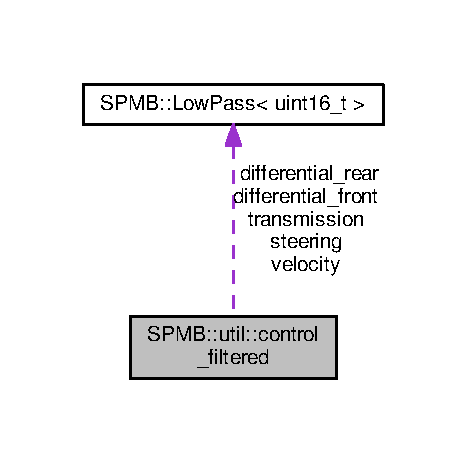
\includegraphics[width=224pt]{structSPMB_1_1util_1_1control__filtered__coll__graph}
\end{center}
\end{figure}
\subsection*{Public Attributes}
\begin{DoxyCompactItemize}
\item 
\hyperlink{classSPMB_1_1LowPass}{Low\+Pass}$<$ uint16\+\_\+t $>$ {\bfseries steering}\hypertarget{structSPMB_1_1util_1_1control__filtered_acfb55895cf3f448daba4805d3c721dae}{}\label{structSPMB_1_1util_1_1control__filtered_acfb55895cf3f448daba4805d3c721dae}

\item 
\hyperlink{classSPMB_1_1LowPass}{Low\+Pass}$<$ uint16\+\_\+t $>$ {\bfseries velocity}\hypertarget{structSPMB_1_1util_1_1control__filtered_a5aef24fc07fad743734bb36fffe0ee16}{}\label{structSPMB_1_1util_1_1control__filtered_a5aef24fc07fad743734bb36fffe0ee16}

\item 
\hyperlink{classSPMB_1_1LowPass}{Low\+Pass}$<$ uint16\+\_\+t $>$ {\bfseries transmission}\hypertarget{structSPMB_1_1util_1_1control__filtered_ad64df625235662b019cc11f7b5e8c555}{}\label{structSPMB_1_1util_1_1control__filtered_ad64df625235662b019cc11f7b5e8c555}

\item 
\hyperlink{classSPMB_1_1LowPass}{Low\+Pass}$<$ uint16\+\_\+t $>$ {\bfseries differential\+\_\+front}\hypertarget{structSPMB_1_1util_1_1control__filtered_ac5678602b91470ee02f848c155036f5f}{}\label{structSPMB_1_1util_1_1control__filtered_ac5678602b91470ee02f848c155036f5f}

\item 
\hyperlink{classSPMB_1_1LowPass}{Low\+Pass}$<$ uint16\+\_\+t $>$ {\bfseries differential\+\_\+rear}\hypertarget{structSPMB_1_1util_1_1control__filtered_a619aa50937200c894bb3dc0478ab58bd}{}\label{structSPMB_1_1util_1_1control__filtered_a619aa50937200c894bb3dc0478ab58bd}

\end{DoxyCompactItemize}


\subsection{Detailed Description}


Definition at line 24 of file util.\+h.


\hypertarget{classSPMB_1_1InterruptGroup}{}\section{S\+P\+MB\+:\+:Interrupt\+Group Class Reference}
\label{classSPMB_1_1InterruptGroup}\index{S\+P\+M\+B\+::\+Interrupt\+Group@{S\+P\+M\+B\+::\+Interrupt\+Group}}


Collects Interrupts with same properties in groups and.  




{\ttfamily \#include $<$input\+\_\+rc.\+h$>$}



Collaboration diagram for S\+P\+MB\+:\+:Interrupt\+Group\+:\nopagebreak
\begin{figure}[H]
\begin{center}
\leavevmode
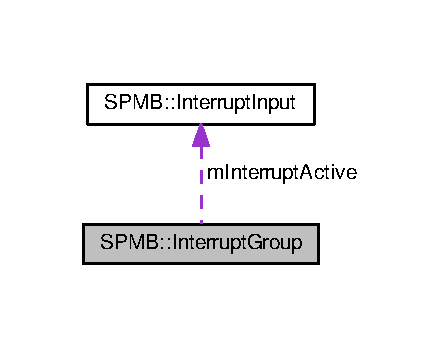
\includegraphics[width=213pt]{classSPMB_1_1InterruptGroup__coll__graph}
\end{center}
\end{figure}
\subsection*{Public Member Functions}
\begin{DoxyCompactItemize}
\item 
\hyperlink{classSPMB_1_1InterruptGroup_ae9b011533b9da5bf30a761a9807a81fd}{Interrupt\+Group} ()\hypertarget{classSPMB_1_1InterruptGroup_ae9b011533b9da5bf30a761a9807a81fd}{}\label{classSPMB_1_1InterruptGroup_ae9b011533b9da5bf30a761a9807a81fd}

\begin{DoxyCompactList}\small\item\em Constructor. \end{DoxyCompactList}\item 
void \hyperlink{classSPMB_1_1InterruptGroup_af657eec701e542ca195e2ac8fe817527}{append\+\_\+interrupt} (\hyperlink{classSPMB_1_1InterruptInput}{Interrupt\+Input} $\ast$New\+Interrupt\+Input)\hypertarget{classSPMB_1_1InterruptGroup_af657eec701e542ca195e2ac8fe817527}{}\label{classSPMB_1_1InterruptGroup_af657eec701e542ca195e2ac8fe817527}

\begin{DoxyCompactList}\small\item\em Append new interrupt to vector. \end{DoxyCompactList}\item 
void \hyperlink{classSPMB_1_1InterruptGroup_a40e413db26817d4381295fbe0cc41f85}{update\+\_\+timer} ()\hypertarget{classSPMB_1_1InterruptGroup_a40e413db26817d4381295fbe0cc41f85}{}\label{classSPMB_1_1InterruptGroup_a40e413db26817d4381295fbe0cc41f85}

\begin{DoxyCompactList}\small\item\em Update timer for each interrupt. \end{DoxyCompactList}\item 
void \hyperlink{classSPMB_1_1InterruptGroup_acb1097331ab9adc74cfc49405d313e94}{\+\_\+attempt\+\_\+rotating} ()\hypertarget{classSPMB_1_1InterruptGroup_acb1097331ab9adc74cfc49405d313e94}{}\label{classSPMB_1_1InterruptGroup_acb1097331ab9adc74cfc49405d313e94}

\begin{DoxyCompactList}\small\item\em Attempt to rotate and search for a good status in one of the interrupts and update skipped interrupts with bad status flag. \end{DoxyCompactList}\item 
void \hyperlink{classSPMB_1_1InterruptGroup_a0636f92ce6b96c7e3c2c93dd8b8352f9}{rotate\+\_\+interrupts} ()\hypertarget{classSPMB_1_1InterruptGroup_a0636f92ce6b96c7e3c2c93dd8b8352f9}{}\label{classSPMB_1_1InterruptGroup_a0636f92ce6b96c7e3c2c93dd8b8352f9}

\begin{DoxyCompactList}\small\item\em Rotate active interrupt to next interrupt in interrupt group with good status flag and update error flags. \end{DoxyCompactList}\end{DoxyCompactItemize}
\subsection*{Public Attributes}
\begin{DoxyCompactItemize}
\item 
volatile uint8\+\_\+t \hyperlink{classSPMB_1_1InterruptGroup_a390d762b5aaa808d07aef963fa5296ed}{m\+Idx}\hypertarget{classSPMB_1_1InterruptGroup_a390d762b5aaa808d07aef963fa5296ed}{}\label{classSPMB_1_1InterruptGroup_a390d762b5aaa808d07aef963fa5296ed}

\begin{DoxyCompactList}\small\item\em Index for current iterated interrupt  replace with iterators. \end{DoxyCompactList}\item 
std\+::vector$<$ \hyperlink{classSPMB_1_1InterruptInput}{Interrupt\+Input} $\ast$ $>$ \hyperlink{classSPMB_1_1InterruptGroup_a0eff897d66e69f20cbc4c83d05a64293}{m\+Interrupts}\hypertarget{classSPMB_1_1InterruptGroup_a0eff897d66e69f20cbc4c83d05a64293}{}\label{classSPMB_1_1InterruptGroup_a0eff897d66e69f20cbc4c83d05a64293}

\begin{DoxyCompactList}\small\item\em Interrupt pountires. \end{DoxyCompactList}\item 
\hyperlink{classSPMB_1_1InterruptInput}{Interrupt\+Input} $\ast$ \hyperlink{classSPMB_1_1InterruptGroup_a894e60cb901974f3b2731c5638245340}{m\+Interrupt\+Active}\hypertarget{classSPMB_1_1InterruptGroup_a894e60cb901974f3b2731c5638245340}{}\label{classSPMB_1_1InterruptGroup_a894e60cb901974f3b2731c5638245340}

\begin{DoxyCompactList}\small\item\em Pointer to current interrupt. \end{DoxyCompactList}\end{DoxyCompactItemize}


\subsection{Detailed Description}
Collects Interrupts with same properties in groups and. 

Definition at line 59 of file input\+\_\+rc.\+h.


\hypertarget{classSPMB_1_1InterruptInput}{}\section{S\+P\+MB\+:\+:Interrupt\+Input Class Reference}
\label{classSPMB_1_1InterruptInput}\index{S\+P\+M\+B\+::\+Interrupt\+Input@{S\+P\+M\+B\+::\+Interrupt\+Input}}


Collection of all register necessary for interfacing with an interrupt pin.  




{\ttfamily \#include $<$input\+\_\+rc.\+h$>$}

\subsection*{Public Member Functions}
\begin{DoxyCompactItemize}
\item 
\hyperlink{classSPMB_1_1InterruptInput_a1d7054c59edcd2989088eda0d6615370}{Interrupt\+Input} ()\hypertarget{classSPMB_1_1InterruptInput_a1d7054c59edcd2989088eda0d6615370}{}\label{classSPMB_1_1InterruptInput_a1d7054c59edcd2989088eda0d6615370}

\begin{DoxyCompactList}\small\item\em Default Constructor. \end{DoxyCompactList}\item 
void \hyperlink{classSPMB_1_1InterruptInput_a537b9601886237322cd01b4d66a1cae3}{initialise} (std\+::string label\+Input\+\_\+, uint16\+\_\+t Default\+Time\+Period\+\_\+, uint8\+\_\+t Bit\+Input\+\_\+, volatile uint8\+\_\+t $\ast$Direction\+Register\+\_\+, volatile uint8\+\_\+t $\ast$Cfg\+Register\+\_\+, volatile uint8\+\_\+t $\ast$Data\+Register\+\_\+, volatile uint8\+\_\+t $\ast$Interrupt\+Register\+\_\+)\hypertarget{classSPMB_1_1InterruptInput_a537b9601886237322cd01b4d66a1cae3}{}\label{classSPMB_1_1InterruptInput_a537b9601886237322cd01b4d66a1cae3}

\begin{DoxyCompactList}\small\item\em Parse register arguments to member variables. \end{DoxyCompactList}\item 
void \hyperlink{classSPMB_1_1InterruptInput_af458652456481ec1ee7af3381f4df732}{configure} ()\hypertarget{classSPMB_1_1InterruptInput_af458652456481ec1ee7af3381f4df732}{}\label{classSPMB_1_1InterruptInput_af458652456481ec1ee7af3381f4df732}

\begin{DoxyCompactList}\small\item\em Takes care of setting up all the pins for input definitions and pull-\/up configuration of respective pin. \end{DoxyCompactList}\item 
void \hyperlink{classSPMB_1_1InterruptInput_a434a4a22e379f9d3e70340ca638ef0d9}{disarm\+\_\+interrupt} ()\hypertarget{classSPMB_1_1InterruptInput_a434a4a22e379f9d3e70340ca638ef0d9}{}\label{classSPMB_1_1InterruptInput_a434a4a22e379f9d3e70340ca638ef0d9}

\begin{DoxyCompactList}\small\item\em Disarms the Pin for Pin Change Interrupts. \end{DoxyCompactList}\item 
void \hyperlink{classSPMB_1_1InterruptInput_a6f677f7648a3252791ab61df4c5e64b6}{arm\+\_\+interrupt} ()\hypertarget{classSPMB_1_1InterruptInput_a6f677f7648a3252791ab61df4c5e64b6}{}\label{classSPMB_1_1InterruptInput_a6f677f7648a3252791ab61df4c5e64b6}

\begin{DoxyCompactList}\small\item\em Arms the Pin for Pin Change Interrupts. \end{DoxyCompactList}\item 
void \hyperlink{classSPMB_1_1InterruptInput_af827e44330f1054bdfdb28861dbd6505}{update\+\_\+timer} ()\hypertarget{classSPMB_1_1InterruptInput_af827e44330f1054bdfdb28861dbd6505}{}\label{classSPMB_1_1InterruptInput_af827e44330f1054bdfdb28861dbd6505}

\begin{DoxyCompactList}\small\item\em Handles complete interrupt logic (is called by \hyperlink{classSPMB_1_1InterruptManager}{Interrupt\+Manager}) \end{DoxyCompactList}\item 
void \hyperlink{classSPMB_1_1InterruptInput_a454efe88ea6a9c5047e5c34b9d1f7e4b}{switch\+\_\+error\+\_\+status} ()\hypertarget{classSPMB_1_1InterruptInput_a454efe88ea6a9c5047e5c34b9d1f7e4b}{}\label{classSPMB_1_1InterruptInput_a454efe88ea6a9c5047e5c34b9d1f7e4b}

\begin{DoxyCompactList}\small\item\em Checks whether to reenable or to disable a interrupt with a certain error trigger count. \end{DoxyCompactList}\item 
void \hyperlink{classSPMB_1_1InterruptInput_adb38e98b59d2c4487bedd00eba453ab2}{reset} ()\hypertarget{classSPMB_1_1InterruptInput_adb38e98b59d2c4487bedd00eba453ab2}{}\label{classSPMB_1_1InterruptInput_adb38e98b59d2c4487bedd00eba453ab2}

\begin{DoxyCompactList}\small\item\em Reset Interrupt. \end{DoxyCompactList}\end{DoxyCompactItemize}
\subsection*{Public Attributes}
\begin{DoxyCompactItemize}
\item 
std\+::string \hyperlink{classSPMB_1_1InterruptInput_ad07b7faae89412b9cbeb138efd0fb091}{m\+Label}\hypertarget{classSPMB_1_1InterruptInput_ad07b7faae89412b9cbeb138efd0fb091}{}\label{classSPMB_1_1InterruptInput_ad07b7faae89412b9cbeb138efd0fb091}

\begin{DoxyCompactList}\small\item\em Label identifier for searching interrupt with interrupt manager. \end{DoxyCompactList}\item 
volatile uint8\+\_\+t \hyperlink{classSPMB_1_1InterruptInput_a1c093ecf08a4b18066a61abb0cd9b783}{m\+Bit}\hypertarget{classSPMB_1_1InterruptInput_a1c093ecf08a4b18066a61abb0cd9b783}{}\label{classSPMB_1_1InterruptInput_a1c093ecf08a4b18066a61abb0cd9b783}

\begin{DoxyCompactList}\small\item\em Bit number in Register. \end{DoxyCompactList}\item 
volatile uint8\+\_\+t $\ast$ \hyperlink{classSPMB_1_1InterruptInput_a31b05aaa064545e134c6a158cfbcd5f3}{m\+Data\+Register}\hypertarget{classSPMB_1_1InterruptInput_a31b05aaa064545e134c6a158cfbcd5f3}{}\label{classSPMB_1_1InterruptInput_a31b05aaa064545e134c6a158cfbcd5f3}

\begin{DoxyCompactList}\small\item\em Data register for corresponding interrupt and providing the pin value. \end{DoxyCompactList}\item 
volatile uint8\+\_\+t $\ast$ \hyperlink{classSPMB_1_1InterruptInput_a0bc9e2864357842924edf1f7bb619754}{m\+Direction\+Register}\hypertarget{classSPMB_1_1InterruptInput_a0bc9e2864357842924edf1f7bb619754}{}\label{classSPMB_1_1InterruptInput_a0bc9e2864357842924edf1f7bb619754}

\begin{DoxyCompactList}\small\item\em Direction register defining the pin as either an input (0) or output (1) \end{DoxyCompactList}\item 
volatile uint8\+\_\+t $\ast$ \hyperlink{classSPMB_1_1InterruptInput_a9529d56cc9ec75b1977bad24ad28ec77}{m\+Cfg\+Register}\hypertarget{classSPMB_1_1InterruptInput_a9529d56cc9ec75b1977bad24ad28ec77}{}\label{classSPMB_1_1InterruptInput_a9529d56cc9ec75b1977bad24ad28ec77}

\begin{DoxyCompactList}\small\item\em Configuration register providing the option to activate pull-\/ups (1) and no pull-\/ups (0) \end{DoxyCompactList}\item 
volatile uint8\+\_\+t $\ast$ \hyperlink{classSPMB_1_1InterruptInput_a3170d37b09700931f4d5eecdc03fd623}{m\+Interrupt\+Register}\hypertarget{classSPMB_1_1InterruptInput_a3170d37b09700931f4d5eecdc03fd623}{}\label{classSPMB_1_1InterruptInput_a3170d37b09700931f4d5eecdc03fd623}

\begin{DoxyCompactList}\small\item\em Interrupt activation register, enables the Bit\textquotesingle{}s interrupt. \end{DoxyCompactList}\item 
volatile long \hyperlink{classSPMB_1_1InterruptInput_a7ed0aa1999b25c9ecb5f475915621d6e}{m\+Timer}\hypertarget{classSPMB_1_1InterruptInput_a7ed0aa1999b25c9ecb5f475915621d6e}{}\label{classSPMB_1_1InterruptInput_a7ed0aa1999b25c9ecb5f475915621d6e}

\begin{DoxyCompactList}\small\item\em Timestamp variable for last interrupt activation. \end{DoxyCompactList}\item 
volatile uint16\+\_\+t \hyperlink{classSPMB_1_1InterruptInput_aea7eb654589b9835f2ce5a9a837de266}{m\+Time\+Period\+Valid}\hypertarget{classSPMB_1_1InterruptInput_aea7eb654589b9835f2ce5a9a837de266}{}\label{classSPMB_1_1InterruptInput_aea7eb654589b9835f2ce5a9a837de266}

\begin{DoxyCompactList}\small\item\em Intermediary variable for always storing only accepted time periods. \end{DoxyCompactList}\item 
volatile uint16\+\_\+t \hyperlink{classSPMB_1_1InterruptInput_aa1149ffe5132907852832825696d4a79}{m\+Time\+Period}\hypertarget{classSPMB_1_1InterruptInput_aa1149ffe5132907852832825696d4a79}{}\label{classSPMB_1_1InterruptInput_aa1149ffe5132907852832825696d4a79}

\begin{DoxyCompactList}\small\item\em Temporary and volatile time period variable that can contain erroneous reads. \end{DoxyCompactList}\item 
volatile uint16\+\_\+t \hyperlink{classSPMB_1_1InterruptInput_ae479068bfc0e3dec59ed0828e78129bc}{m\+Time\+Period\+Default}\hypertarget{classSPMB_1_1InterruptInput_ae479068bfc0e3dec59ed0828e78129bc}{}\label{classSPMB_1_1InterruptInput_ae479068bfc0e3dec59ed0828e78129bc}

\begin{DoxyCompactList}\small\item\em Default time period as substitution of erroneous reads as output in case of errors. \end{DoxyCompactList}\item 
volatile bool \hyperlink{classSPMB_1_1InterruptInput_a0221d38d44c3a9dc32a7d33d217d8e59}{m\+Status}\hypertarget{classSPMB_1_1InterruptInput_a0221d38d44c3a9dc32a7d33d217d8e59}{}\label{classSPMB_1_1InterruptInput_a0221d38d44c3a9dc32a7d33d217d8e59}

\begin{DoxyCompactList}\small\item\em Status boolean, showing good (true) or bad status (false) of interrupt. \end{DoxyCompactList}\item 
volatile bool \hyperlink{classSPMB_1_1InterruptInput_aeb0a16f69fd343042fed1d56abb44d2d}{m\+Received\+High}\hypertarget{classSPMB_1_1InterruptInput_aeb0a16f69fd343042fed1d56abb44d2d}{}\label{classSPMB_1_1InterruptInput_aeb0a16f69fd343042fed1d56abb44d2d}

\begin{DoxyCompactList}\small\item\em Indicator that a high pin level has been read. Only possible after low read. \end{DoxyCompactList}\item 
volatile bool \hyperlink{classSPMB_1_1InterruptInput_aab7e3304495e1ee98d812157368091e5}{m\+Received\+Low}\hypertarget{classSPMB_1_1InterruptInput_aab7e3304495e1ee98d812157368091e5}{}\label{classSPMB_1_1InterruptInput_aab7e3304495e1ee98d812157368091e5}

\begin{DoxyCompactList}\small\item\em Indicator that a low value has been read. \end{DoxyCompactList}\item 
volatile bool \hyperlink{classSPMB_1_1InterruptInput_a6824c0d5fae32571df02ea13aa2f8802}{m\+New\+Interrupt\+Available}\hypertarget{classSPMB_1_1InterruptInput_a6824c0d5fae32571df02ea13aa2f8802}{}\label{classSPMB_1_1InterruptInput_a6824c0d5fae32571df02ea13aa2f8802}

\begin{DoxyCompactList}\small\item\em Indicator that a complete cycle has been observed and that pin is disarmed. \end{DoxyCompactList}\item 
volatile uint8\+\_\+t \hyperlink{classSPMB_1_1InterruptInput_a76da8c6e70323bdfd0219f63e23529e8}{m\+Error\+Count}\hypertarget{classSPMB_1_1InterruptInput_a76da8c6e70323bdfd0219f63e23529e8}{}\label{classSPMB_1_1InterruptInput_a76da8c6e70323bdfd0219f63e23529e8}

\begin{DoxyCompactList}\small\item\em Statistic about both the negative errors (when to disable with m\+Status false) as well as the amount the interrupt has been ignored in rotation and when it is time to turn back on (m\+Status true). \end{DoxyCompactList}\end{DoxyCompactItemize}


\subsection{Detailed Description}
Collection of all register necessary for interfacing with an interrupt pin. 

Definition at line 7 of file input\+\_\+rc.\+h.


\hypertarget{classSPMB_1_1InterruptManager}{}\section{S\+P\+MB\+:\+:Interrupt\+Manager Class Reference}
\label{classSPMB_1_1InterruptManager}\index{S\+P\+M\+B\+::\+Interrupt\+Manager@{S\+P\+M\+B\+::\+Interrupt\+Manager}}


Collection of Interrupt Groups (e.\+g. sorted as time sensitive and non-\/time sensitive ).  




{\ttfamily \#include $<$input\+\_\+rc.\+h$>$}

\subsection*{Public Member Functions}
\begin{DoxyCompactItemize}
\item 
void \hyperlink{classSPMB_1_1InterruptManager_a7848e944d851bf3bcc251e03e673433c}{append\+\_\+group} (\hyperlink{classSPMB_1_1InterruptGroup}{Interrupt\+Group} $\ast$new\+Interrupt\+Group)\hypertarget{classSPMB_1_1InterruptManager_a7848e944d851bf3bcc251e03e673433c}{}\label{classSPMB_1_1InterruptManager_a7848e944d851bf3bcc251e03e673433c}

\begin{DoxyCompactList}\small\item\em Append a new interrupt group to the interrupt manager. \end{DoxyCompactList}\item 
void \hyperlink{classSPMB_1_1InterruptManager_a281ff95c62f2c714024009fbdfad560e}{rotate\+\_\+interrupts} ()\hypertarget{classSPMB_1_1InterruptManager_a281ff95c62f2c714024009fbdfad560e}{}\label{classSPMB_1_1InterruptManager_a281ff95c62f2c714024009fbdfad560e}

\begin{DoxyCompactList}\small\item\em Rotate all interrupts or attempt to rotate in case some are idle or in an erroneous state. \end{DoxyCompactList}\item 
void \hyperlink{classSPMB_1_1InterruptManager_ae6d936207409563b307e3f0bbced7dbc}{arm\+\_\+interrupts} ()\hypertarget{classSPMB_1_1InterruptManager_ae6d936207409563b307e3f0bbced7dbc}{}\label{classSPMB_1_1InterruptManager_ae6d936207409563b307e3f0bbced7dbc}

\begin{DoxyCompactList}\small\item\em Arm all interrupts. \end{DoxyCompactList}\item 
bool \hyperlink{classSPMB_1_1InterruptManager_abef4d7dfc94ed70cb9b137803d75ebe4}{get\+\_\+time\+\_\+period} (std\+::string label, volatile uint16\+\_\+t \&time\+\_\+period)\hypertarget{classSPMB_1_1InterruptManager_abef4d7dfc94ed70cb9b137803d75ebe4}{}\label{classSPMB_1_1InterruptManager_abef4d7dfc94ed70cb9b137803d75ebe4}

\begin{DoxyCompactList}\small\item\em Get time period for a interrupt identified with the provided label argument and store result in time\+\_\+period argument. \end{DoxyCompactList}\end{DoxyCompactItemize}
\subsection*{Public Attributes}
\begin{DoxyCompactItemize}
\item 
std\+::vector$<$ \hyperlink{classSPMB_1_1InterruptGroup}{Interrupt\+Group} $\ast$ $>$ \hyperlink{classSPMB_1_1InterruptManager_a103e2348c57eecaab0605c196f3b924b}{m\+Interrupt\+Groups}\hypertarget{classSPMB_1_1InterruptManager_a103e2348c57eecaab0605c196f3b924b}{}\label{classSPMB_1_1InterruptManager_a103e2348c57eecaab0605c196f3b924b}

\begin{DoxyCompactList}\small\item\em $<$ Collection of all interrupt groups storing their pointers. \end{DoxyCompactList}\end{DoxyCompactItemize}


\subsection{Detailed Description}
Collection of Interrupt Groups (e.\+g. sorted as time sensitive and non-\/time sensitive ). 

Definition at line 119 of file input\+\_\+rc.\+h.


\hypertarget{classSPMB_1_1LowPass}{}\section{S\+P\+MB\+:\+:Low\+Pass$<$ T $>$ Class Template Reference}
\label{classSPMB_1_1LowPass}\index{S\+P\+M\+B\+::\+Low\+Pass$<$ T $>$@{S\+P\+M\+B\+::\+Low\+Pass$<$ T $>$}}


{\ttfamily \#include $<$lowpass.\+h$>$}



Collaboration diagram for S\+P\+MB\+:\+:Low\+Pass$<$ T $>$\+:
\nopagebreak
\begin{figure}[H]
\begin{center}
\leavevmode
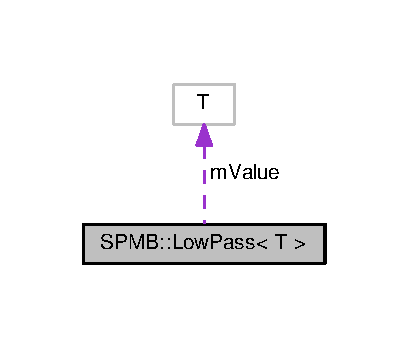
\includegraphics[width=196pt]{classSPMB_1_1LowPass__coll__graph}
\end{center}
\end{figure}
\subsection*{Public Member Functions}
\begin{DoxyCompactItemize}
\item 
void \hyperlink{classSPMB_1_1LowPass_a11696a906cb869ccf580673b8ddfee3b}{\+\_\+correct\+\_\+period} (volatile uint16\+\_\+t \&period\+\_\+corrected)
\item 
void \hyperlink{classSPMB_1_1LowPass_ac01c87236e0a4974e0fe63c648ad0a7e}{update\+\_\+state} (T New\+State)
\item 
T \hyperlink{classSPMB_1_1LowPass_a5f21ff8ce24fcbd7296edd991b425556}{value} ()
\item 
{\bfseries Low\+Pass} (float time\+\_\+constant\+\_\+in\+\_\+seconds, T default\+\_\+value)\hypertarget{classSPMB_1_1LowPass_a763169e42d8a7059a77a6fda0ae98f24}{}\label{classSPMB_1_1LowPass_a763169e42d8a7059a77a6fda0ae98f24}

\end{DoxyCompactItemize}
\subsection*{Public Attributes}
\begin{DoxyCompactItemize}
\item 
uint16\+\_\+t \hyperlink{classSPMB_1_1LowPass_a3272be66039cc317ae295f7e4ce90c23}{m\+Time\+Constant}
\item 
long \hyperlink{classSPMB_1_1LowPass_a0d65cef27970b458eb9a8065e3141eae}{m\+Timestamp}
\item 
T \hyperlink{classSPMB_1_1LowPass_a63f1e9ef7ccb4a1b51ebb81681d377ec}{m\+Value}
\end{DoxyCompactItemize}


\subsection{Detailed Description}
\subsubsection*{template$<$typename T$>$\\*
class S\+P\+M\+B\+::\+Low\+Pass$<$ T $>$}

class 

Definition at line 9 of file lowpass.\+h.



\subsection{Member Function Documentation}
\index{S\+P\+M\+B\+::\+Low\+Pass@{S\+P\+M\+B\+::\+Low\+Pass}!\+\_\+correct\+\_\+period@{\+\_\+correct\+\_\+period}}
\index{\+\_\+correct\+\_\+period@{\+\_\+correct\+\_\+period}!S\+P\+M\+B\+::\+Low\+Pass@{S\+P\+M\+B\+::\+Low\+Pass}}
\subsubsection[{\texorpdfstring{\+\_\+correct\+\_\+period(volatile uint16\+\_\+t \&period\+\_\+corrected)}{_correct_period(volatile uint16_t &period_corrected)}}]{\setlength{\rightskip}{0pt plus 5cm}template$<$typename T $>$ void {\bf S\+P\+M\+B\+::\+Low\+Pass}$<$ T $>$\+::\+\_\+correct\+\_\+period (
\begin{DoxyParamCaption}
\item[{volatile uint16\+\_\+t \&}]{period\+\_\+corrected}
\end{DoxyParamCaption}
)}\hypertarget{classSPMB_1_1LowPass_a11696a906cb869ccf580673b8ddfee3b}{}\label{classSPMB_1_1LowPass_a11696a906cb869ccf580673b8ddfee3b}
aeu 

Definition at line 27 of file lowpass.\+h.

\index{S\+P\+M\+B\+::\+Low\+Pass@{S\+P\+M\+B\+::\+Low\+Pass}!update\+\_\+state@{update\+\_\+state}}
\index{update\+\_\+state@{update\+\_\+state}!S\+P\+M\+B\+::\+Low\+Pass@{S\+P\+M\+B\+::\+Low\+Pass}}
\subsubsection[{\texorpdfstring{update\+\_\+state(\+T New\+State)}{update_state(T NewState)}}]{\setlength{\rightskip}{0pt plus 5cm}template$<$typename T$>$ void {\bf S\+P\+M\+B\+::\+Low\+Pass}$<$ T $>$\+::update\+\_\+state (
\begin{DoxyParamCaption}
\item[{T}]{New\+State}
\end{DoxyParamCaption}
)}\hypertarget{classSPMB_1_1LowPass_ac01c87236e0a4974e0fe63c648ad0a7e}{}\label{classSPMB_1_1LowPass_ac01c87236e0a4974e0fe63c648ad0a7e}
aoeu 

Definition at line 52 of file lowpass.\+h.

\index{S\+P\+M\+B\+::\+Low\+Pass@{S\+P\+M\+B\+::\+Low\+Pass}!value@{value}}
\index{value@{value}!S\+P\+M\+B\+::\+Low\+Pass@{S\+P\+M\+B\+::\+Low\+Pass}}
\subsubsection[{\texorpdfstring{value()}{value()}}]{\setlength{\rightskip}{0pt plus 5cm}template$<$typename T $>$ T {\bf S\+P\+M\+B\+::\+Low\+Pass}$<$ T $>$\+::value (
\begin{DoxyParamCaption}
{}
\end{DoxyParamCaption}
)}\hypertarget{classSPMB_1_1LowPass_a5f21ff8ce24fcbd7296edd991b425556}{}\label{classSPMB_1_1LowPass_a5f21ff8ce24fcbd7296edd991b425556}
eaou 

Definition at line 40 of file lowpass.\+h.



\subsection{Member Data Documentation}
\index{S\+P\+M\+B\+::\+Low\+Pass@{S\+P\+M\+B\+::\+Low\+Pass}!m\+Time\+Constant@{m\+Time\+Constant}}
\index{m\+Time\+Constant@{m\+Time\+Constant}!S\+P\+M\+B\+::\+Low\+Pass@{S\+P\+M\+B\+::\+Low\+Pass}}
\subsubsection[{\texorpdfstring{m\+Time\+Constant}{mTimeConstant}}]{\setlength{\rightskip}{0pt plus 5cm}template$<$typename T$>$ uint16\+\_\+t {\bf S\+P\+M\+B\+::\+Low\+Pass}$<$ T $>$\+::m\+Time\+Constant}\hypertarget{classSPMB_1_1LowPass_a3272be66039cc317ae295f7e4ce90c23}{}\label{classSPMB_1_1LowPass_a3272be66039cc317ae295f7e4ce90c23}
filter constant 

Definition at line 11 of file lowpass.\+h.

\index{S\+P\+M\+B\+::\+Low\+Pass@{S\+P\+M\+B\+::\+Low\+Pass}!m\+Timestamp@{m\+Timestamp}}
\index{m\+Timestamp@{m\+Timestamp}!S\+P\+M\+B\+::\+Low\+Pass@{S\+P\+M\+B\+::\+Low\+Pass}}
\subsubsection[{\texorpdfstring{m\+Timestamp}{mTimestamp}}]{\setlength{\rightskip}{0pt plus 5cm}template$<$typename T$>$ long {\bf S\+P\+M\+B\+::\+Low\+Pass}$<$ T $>$\+::m\+Timestamp}\hypertarget{classSPMB_1_1LowPass_a0d65cef27970b458eb9a8065e3141eae}{}\label{classSPMB_1_1LowPass_a0d65cef27970b458eb9a8065e3141eae}
timestamp since last update 

Definition at line 12 of file lowpass.\+h.

\index{S\+P\+M\+B\+::\+Low\+Pass@{S\+P\+M\+B\+::\+Low\+Pass}!m\+Value@{m\+Value}}
\index{m\+Value@{m\+Value}!S\+P\+M\+B\+::\+Low\+Pass@{S\+P\+M\+B\+::\+Low\+Pass}}
\subsubsection[{\texorpdfstring{m\+Value}{mValue}}]{\setlength{\rightskip}{0pt plus 5cm}template$<$typename T$>$ T {\bf S\+P\+M\+B\+::\+Low\+Pass}$<$ T $>$\+::m\+Value}\hypertarget{classSPMB_1_1LowPass_a63f1e9ef7ccb4a1b51ebb81681d377ec}{}\label{classSPMB_1_1LowPass_a63f1e9ef7ccb4a1b51ebb81681d377ec}
most recent value after last filter update 

Definition at line 13 of file lowpass.\+h.


\hypertarget{classSPMB_1_1OutputDriverI2C}{}\section{S\+P\+MB\+:\+:Output\+Driver\+I2C Class Reference}
\label{classSPMB_1_1OutputDriverI2C}\index{S\+P\+M\+B\+::\+Output\+Driver\+I2C@{S\+P\+M\+B\+::\+Output\+Driver\+I2C}}


Output driver using I2C via P\+C\+A9688.  




{\ttfamily \#include $<$output\+\_\+i2c.\+h$>$}

\subsection*{Public Member Functions}
\begin{DoxyCompactItemize}
\item 
void \hyperlink{classSPMB_1_1OutputDriverI2C_a65b12f0a0b98851d21ad863fd1584725}{configure} ()
\item 
void \hyperlink{classSPMB_1_1OutputDriverI2C_a8b82addf2f9101b22cf8bfca160132cb}{actuate} (\hyperlink{structSPMB_1_1util_1_1control__filtered}{util\+::control\+\_\+filtered} $\ast$output)
\end{DoxyCompactItemize}
\subsection*{Public Attributes}
\begin{DoxyCompactItemize}
\item 
double \hyperlink{classSPMB_1_1OutputDriverI2C_a1dc1d614d4e099105b124656a871aa83}{m\+Us\+Bit}\hypertarget{classSPMB_1_1OutputDriverI2C_a1dc1d614d4e099105b124656a871aa83}{}\label{classSPMB_1_1OutputDriverI2C_a1dc1d614d4e099105b124656a871aa83}

\begin{DoxyCompactList}\small\item\em $<$ Amount of microseconds per bit of 4096 bits total resolution \end{DoxyCompactList}\item 
double \hyperlink{classSPMB_1_1OutputDriverI2C_a8ab5bd3883d50cca560313b5275b81e5}{m\+Offset\+Driver}\hypertarget{classSPMB_1_1OutputDriverI2C_a8ab5bd3883d50cca560313b5275b81e5}{}\label{classSPMB_1_1OutputDriverI2C_a8ab5bd3883d50cca560313b5275b81e5}

\begin{DoxyCompactList}\small\item\em Compensation of output driver period deviation from input in microseconds. \end{DoxyCompactList}\item 
Adafruit\+\_\+\+P\+W\+M\+Servo\+Driver \hyperlink{classSPMB_1_1OutputDriverI2C_aecd74104de6faf86afbc9c1f9cd0b50a}{m\+Driver}\hypertarget{classSPMB_1_1OutputDriverI2C_aecd74104de6faf86afbc9c1f9cd0b50a}{}\label{classSPMB_1_1OutputDriverI2C_aecd74104de6faf86afbc9c1f9cd0b50a}

\begin{DoxyCompactList}\small\item\em Adafruit driver to interface with timer chip. \end{DoxyCompactList}\end{DoxyCompactItemize}


\subsection{Detailed Description}
Output driver using I2C via P\+C\+A9688. 

Definition at line 10 of file output\+\_\+i2c.\+h.



\subsection{Member Function Documentation}
\index{S\+P\+M\+B\+::\+Output\+Driver\+I2C@{S\+P\+M\+B\+::\+Output\+Driver\+I2C}!actuate@{actuate}}
\index{actuate@{actuate}!S\+P\+M\+B\+::\+Output\+Driver\+I2C@{S\+P\+M\+B\+::\+Output\+Driver\+I2C}}
\subsubsection[{\texorpdfstring{actuate(util\+::control\+\_\+filtered $\ast$output)}{actuate(util::control_filtered *output)}}]{\setlength{\rightskip}{0pt plus 5cm}void S\+P\+M\+B\+::\+Output\+Driver\+I2\+C\+::actuate (
\begin{DoxyParamCaption}
\item[{{\bf util\+::control\+\_\+filtered} $\ast$}]{output}
\end{DoxyParamCaption}
)}\hypertarget{classSPMB_1_1OutputDriverI2C_a8b82addf2f9101b22cf8bfca160132cb}{}\label{classSPMB_1_1OutputDriverI2C_a8b82addf2f9101b22cf8bfca160132cb}
send periods to be actuated 

Definition at line 17 of file output\+\_\+i2c.\+cpp.

\index{S\+P\+M\+B\+::\+Output\+Driver\+I2C@{S\+P\+M\+B\+::\+Output\+Driver\+I2C}!configure@{configure}}
\index{configure@{configure}!S\+P\+M\+B\+::\+Output\+Driver\+I2C@{S\+P\+M\+B\+::\+Output\+Driver\+I2C}}
\subsubsection[{\texorpdfstring{configure()}{configure()}}]{\setlength{\rightskip}{0pt plus 5cm}void S\+P\+M\+B\+::\+Output\+Driver\+I2\+C\+::configure (
\begin{DoxyParamCaption}
{}
\end{DoxyParamCaption}
)}\hypertarget{classSPMB_1_1OutputDriverI2C_a65b12f0a0b98851d21ad863fd1584725}{}\label{classSPMB_1_1OutputDriverI2C_a65b12f0a0b98851d21ad863fd1584725}
configure pins and frequencies 

Definition at line 5 of file output\+\_\+i2c.\+cpp.


\hypertarget{classSPMB_1_1ROSInterface}{}\section{S\+P\+MB\+:\+:R\+O\+S\+Interface$<$ T $>$ Class Template Reference}
\label{classSPMB_1_1ROSInterface}\index{S\+P\+M\+B\+::\+R\+O\+S\+Interface$<$ T $>$@{S\+P\+M\+B\+::\+R\+O\+S\+Interface$<$ T $>$}}


{\ttfamily \#include $<$ros\+\_\+interface.\+h$>$}



Collaboration diagram for S\+P\+MB\+:\+:R\+O\+S\+Interface$<$ T $>$\+:
\nopagebreak
\begin{figure}[H]
\begin{center}
\leavevmode
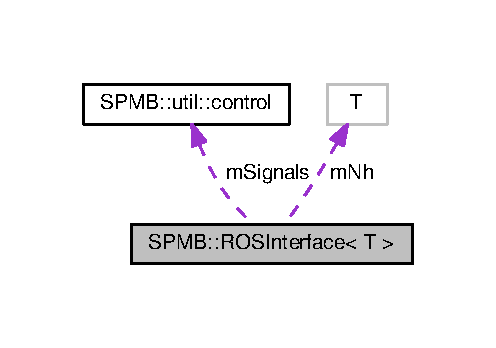
\includegraphics[width=238pt]{classSPMB_1_1ROSInterface__coll__graph}
\end{center}
\end{figure}
\subsection*{Public Member Functions}
\begin{DoxyCompactItemize}
\item 
\hyperlink{classSPMB_1_1ROSInterface_a35478a3b15d22289c6820e70e5cec671}{R\+O\+S\+Interface} (const char $\ast$subscriber\+\_\+topic, const char $\ast$publisher\+\_\+topic)\hypertarget{classSPMB_1_1ROSInterface_a35478a3b15d22289c6820e70e5cec671}{}\label{classSPMB_1_1ROSInterface_a35478a3b15d22289c6820e70e5cec671}

\begin{DoxyCompactList}\small\item\em Constructor. \end{DoxyCompactList}\item 
void \hyperlink{classSPMB_1_1ROSInterface_a24592b40d99ca3ed071b8ef9ab918f4d}{cb\+\_\+request\+\_\+} (const spmbv2\+::request \&msg)
\item 
void \hyperlink{classSPMB_1_1ROSInterface_abb8a72d72e30a8475793200c730e26e6}{publish} (\hyperlink{structSPMB_1_1util_1_1control__filtered}{util\+::control\+\_\+filtered} $\ast$data)
\item 
void \hyperlink{classSPMB_1_1ROSInterface_a6e220ac2a41d61b6185190cc372b1e42}{debug} (const char $\ast$text)
\end{DoxyCompactItemize}
\subsection*{Public Attributes}
\begin{DoxyCompactItemize}
\item 
T {\bfseries m\+Nh}\hypertarget{classSPMB_1_1ROSInterface_a8a0d97d194910287787071f0bba2f874}{}\label{classSPMB_1_1ROSInterface_a8a0d97d194910287787071f0bba2f874}

\item 
spmbv2\+::actuated {\bfseries m\+Msg\+Pub}\hypertarget{classSPMB_1_1ROSInterface_a808aa2a8f9ddeef7a64271ba48886b8e}{}\label{classSPMB_1_1ROSInterface_a808aa2a8f9ddeef7a64271ba48886b8e}

\item 
spmbv2\+::request {\bfseries m\+Msg\+Sub}\hypertarget{classSPMB_1_1ROSInterface_a1c7beeb4a066a0e3810bc17730f21e44}{}\label{classSPMB_1_1ROSInterface_a1c7beeb4a066a0e3810bc17730f21e44}

\item 
\hyperlink{structSPMB_1_1util_1_1control}{util\+::control} {\bfseries m\+Signals}\hypertarget{classSPMB_1_1ROSInterface_ae6913bbbc7b866f368bed451b782e407}{}\label{classSPMB_1_1ROSInterface_ae6913bbbc7b866f368bed451b782e407}

\item 
boolean {\bfseries m\+Is\+Idle}\hypertarget{classSPMB_1_1ROSInterface_a90fe56a55e9599b2d6c87435c3d9fc23}{}\label{classSPMB_1_1ROSInterface_a90fe56a55e9599b2d6c87435c3d9fc23}

\item 
long {\bfseries m\+Timestamp}\hypertarget{classSPMB_1_1ROSInterface_a66af2aff77df71c0e937ce713117cac4}{}\label{classSPMB_1_1ROSInterface_a66af2aff77df71c0e937ce713117cac4}

\item 
uint16\+\_\+t {\bfseries m\+Min\+Time\+Period}\hypertarget{classSPMB_1_1ROSInterface_a7a7df0454febf2d53aab44d82e3e2e15}{}\label{classSPMB_1_1ROSInterface_a7a7df0454febf2d53aab44d82e3e2e15}

\item 
ros\+::\+Subscriber$<$ spmbv2\+::request, \hyperlink{classSPMB_1_1ROSInterface}{R\+O\+S\+Interface}$<$ T $>$ $>$ {\bfseries m\+Subscriber}\hypertarget{classSPMB_1_1ROSInterface_ab24835b7a571abc2ba3c559d94118bf0}{}\label{classSPMB_1_1ROSInterface_ab24835b7a571abc2ba3c559d94118bf0}

\item 
ros\+::\+Publisher {\bfseries m\+Publisher}\hypertarget{classSPMB_1_1ROSInterface_a26a3aac13b059a5fe61d73beb81ca040}{}\label{classSPMB_1_1ROSInterface_a26a3aac13b059a5fe61d73beb81ca040}

\end{DoxyCompactItemize}


\subsection{Detailed Description}
\subsubsection*{template$<$typename T$>$\\*
class S\+P\+M\+B\+::\+R\+O\+S\+Interface$<$ T $>$}

R\+OS Interface class providing interface functions and facilitating publishing and subscribing 

Definition at line 13 of file ros\+\_\+interface.\+h.



\subsection{Member Function Documentation}
\index{S\+P\+M\+B\+::\+R\+O\+S\+Interface@{S\+P\+M\+B\+::\+R\+O\+S\+Interface}!cb\+\_\+request\+\_\+@{cb\+\_\+request\+\_\+}}
\index{cb\+\_\+request\+\_\+@{cb\+\_\+request\+\_\+}!S\+P\+M\+B\+::\+R\+O\+S\+Interface@{S\+P\+M\+B\+::\+R\+O\+S\+Interface}}
\subsubsection[{\texorpdfstring{cb\+\_\+request\+\_\+(const spmbv2\+::request \&msg)}{cb_request_(const spmbv2::request &msg)}}]{\setlength{\rightskip}{0pt plus 5cm}template$<$typename T $>$ void {\bf S\+P\+M\+B\+::\+R\+O\+S\+Interface}$<$ T $>$\+::cb\+\_\+request\+\_\+ (
\begin{DoxyParamCaption}
\item[{const spmbv2\+::request \&}]{msg}
\end{DoxyParamCaption}
)}\hypertarget{classSPMB_1_1ROSInterface_a24592b40d99ca3ed071b8ef9ab918f4d}{}\label{classSPMB_1_1ROSInterface_a24592b40d99ca3ed071b8ef9ab918f4d}
Callback for command request via R\+OS 

Definition at line 41 of file ros\+\_\+interface.\+h.

\index{S\+P\+M\+B\+::\+R\+O\+S\+Interface@{S\+P\+M\+B\+::\+R\+O\+S\+Interface}!debug@{debug}}
\index{debug@{debug}!S\+P\+M\+B\+::\+R\+O\+S\+Interface@{S\+P\+M\+B\+::\+R\+O\+S\+Interface}}
\subsubsection[{\texorpdfstring{debug(const char $\ast$text)}{debug(const char *text)}}]{\setlength{\rightskip}{0pt plus 5cm}template$<$typename T $>$ void {\bf S\+P\+M\+B\+::\+R\+O\+S\+Interface}$<$ T $>$\+::debug (
\begin{DoxyParamCaption}
\item[{const char $\ast$}]{text}
\end{DoxyParamCaption}
)}\hypertarget{classSPMB_1_1ROSInterface_a6e220ac2a41d61b6185190cc372b1e42}{}\label{classSPMB_1_1ROSInterface_a6e220ac2a41d61b6185190cc372b1e42}
Print convenience function for debugging 

Definition at line 52 of file ros\+\_\+interface.\+h.

\index{S\+P\+M\+B\+::\+R\+O\+S\+Interface@{S\+P\+M\+B\+::\+R\+O\+S\+Interface}!publish@{publish}}
\index{publish@{publish}!S\+P\+M\+B\+::\+R\+O\+S\+Interface@{S\+P\+M\+B\+::\+R\+O\+S\+Interface}}
\subsubsection[{\texorpdfstring{publish(util\+::control\+\_\+filtered $\ast$data)}{publish(util::control_filtered *data)}}]{\setlength{\rightskip}{0pt plus 5cm}template$<$typename T $>$ void {\bf S\+P\+M\+B\+::\+R\+O\+S\+Interface}$<$ T $>$\+::publish (
\begin{DoxyParamCaption}
\item[{{\bf util\+::control\+\_\+filtered} $\ast$}]{data}
\end{DoxyParamCaption}
)}\hypertarget{classSPMB_1_1ROSInterface_abb8a72d72e30a8475793200c730e26e6}{}\label{classSPMB_1_1ROSInterface_abb8a72d72e30a8475793200c730e26e6}
Parsing to publish control\+\_\+filtered to R\+OS message actuated 

Definition at line 57 of file ros\+\_\+interface.\+h.


\hypertarget{classSPMB_1_1SetupManager}{}\section{S\+P\+MB\+:\+:Setup\+Manager Class Reference}
\label{classSPMB_1_1SetupManager}\index{S\+P\+M\+B\+::\+Setup\+Manager@{S\+P\+M\+B\+::\+Setup\+Manager}}


Runs the configure script and pin setup for the main classes like \hyperlink{classSPMB_1_1StatusIndicator}{Status\+Indicator}, \hyperlink{classSPMB_1_1InterruptManager}{Interrupt\+Manager} and \hyperlink{classSPMB_1_1OutputDriverI2C}{Output\+Driver\+I2C}.  




{\ttfamily \#include $<$setup.\+h$>$}



Collaboration diagram for S\+P\+MB\+:\+:Setup\+Manager\+:\nopagebreak
\begin{figure}[H]
\begin{center}
\leavevmode
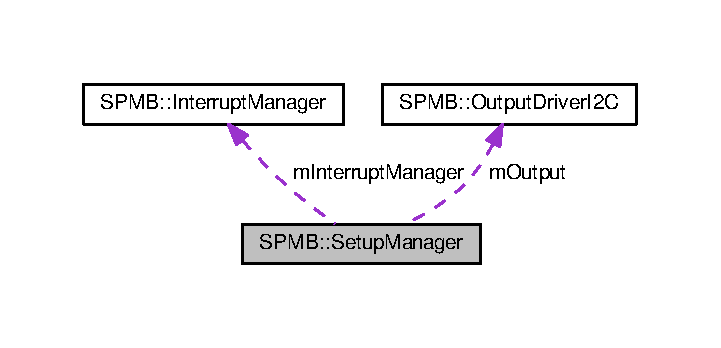
\includegraphics[width=350pt]{classSPMB_1_1SetupManager__coll__graph}
\end{center}
\end{figure}
\subsection*{Public Member Functions}
\begin{DoxyCompactItemize}
\item 
void \hyperlink{classSPMB_1_1SetupManager_ac81e9e0b26c8560fe12ba38f3147bf8d}{delay\+\_\+start} (float seconds\+\_\+to\+\_\+wait)\hypertarget{classSPMB_1_1SetupManager_ac81e9e0b26c8560fe12ba38f3147bf8d}{}\label{classSPMB_1_1SetupManager_ac81e9e0b26c8560fe12ba38f3147bf8d}

\begin{DoxyCompactList}\small\item\em Delay start for initialisation. \end{DoxyCompactList}\item 
void \hyperlink{classSPMB_1_1SetupManager_a1c09eba4b47ad6012b6d3ced131da0a4}{\+\_\+common} ()\hypertarget{classSPMB_1_1SetupManager_a1c09eba4b47ad6012b6d3ced131da0a4}{}\label{classSPMB_1_1SetupManager_a1c09eba4b47ad6012b6d3ced131da0a4}

\begin{DoxyCompactList}\small\item\em Common setup script. \end{DoxyCompactList}\item 
void \hyperlink{classSPMB_1_1SetupManager_ae32219bb0aadfbfa2db519a6ebb58555}{configure\+\_\+common} ()\hypertarget{classSPMB_1_1SetupManager_ae32219bb0aadfbfa2db519a6ebb58555}{}\label{classSPMB_1_1SetupManager_ae32219bb0aadfbfa2db519a6ebb58555}

\begin{DoxyCompactList}\small\item\em Configure more common setup tools. \end{DoxyCompactList}\item 
void \hyperlink{classSPMB_1_1SetupManager_a4a1120a522bf828a08d603ce4982e58d}{configure\+\_\+status\+\_\+indicator} (\hyperlink{classSPMB_1_1StatusIndicator}{Status\+Indicator} $\ast$status\+\_\+indicator\+\_\+in)\hypertarget{classSPMB_1_1SetupManager_a4a1120a522bf828a08d603ce4982e58d}{}\label{classSPMB_1_1SetupManager_a4a1120a522bf828a08d603ce4982e58d}

\begin{DoxyCompactList}\small\item\em Configure status indicator. \end{DoxyCompactList}\item 
void \hyperlink{classSPMB_1_1SetupManager_ad22820d8804c92c80f06c267486f3cc8}{\+\_\+configure\+\_\+interrupts} ()\hypertarget{classSPMB_1_1SetupManager_ad22820d8804c92c80f06c267486f3cc8}{}\label{classSPMB_1_1SetupManager_ad22820d8804c92c80f06c267486f3cc8}

\begin{DoxyCompactList}\small\item\em Configure interrupts by looping through each that is present in interrupt manager.\+n. \end{DoxyCompactList}\item 
void \hyperlink{classSPMB_1_1SetupManager_a5e594557d762d7d7b5141bb1f8cf5227}{configure\+\_\+interrupts} (\hyperlink{classSPMB_1_1InterruptManager}{Interrupt\+Manager} $\ast$interrupt\+\_\+manager\+\_\+in)\hypertarget{classSPMB_1_1SetupManager_a5e594557d762d7d7b5141bb1f8cf5227}{}\label{classSPMB_1_1SetupManager_a5e594557d762d7d7b5141bb1f8cf5227}

\begin{DoxyCompactList}\small\item\em Wrapper around configure interrupts. \end{DoxyCompactList}\item 
void \hyperlink{classSPMB_1_1SetupManager_a4e7be3a3f5e5c073a45f5059d56639eb}{configure\+\_\+output} (\hyperlink{classSPMB_1_1OutputDriverI2C}{Output\+Driver\+I2C} $\ast$output\+\_\+in)\hypertarget{classSPMB_1_1SetupManager_a4e7be3a3f5e5c073a45f5059d56639eb}{}\label{classSPMB_1_1SetupManager_a4e7be3a3f5e5c073a45f5059d56639eb}

\begin{DoxyCompactList}\small\item\em Configure output driver. \end{DoxyCompactList}\item 
void \hyperlink{classSPMB_1_1SetupManager_a3db6edae988d49263fc640148f678d38}{arm\+\_\+system} ()\hypertarget{classSPMB_1_1SetupManager_a3db6edae988d49263fc640148f678d38}{}\label{classSPMB_1_1SetupManager_a3db6edae988d49263fc640148f678d38}

\begin{DoxyCompactList}\small\item\em Arm autonomous system. \end{DoxyCompactList}\item 
\hyperlink{classSPMB_1_1SetupManager_a712e674e38b672f20d5d007e8c64d548}{Setup\+Manager} ()\hypertarget{classSPMB_1_1SetupManager_a712e674e38b672f20d5d007e8c64d548}{}\label{classSPMB_1_1SetupManager_a712e674e38b672f20d5d007e8c64d548}

\begin{DoxyCompactList}\small\item\em Pointer to status\+\_\+indicator for initialisation. \end{DoxyCompactList}\end{DoxyCompactItemize}
\subsection*{Public Attributes}
\begin{DoxyCompactItemize}
\item 
\hyperlink{classSPMB_1_1StatusIndicator}{Status\+Indicator} $\ast$ \hyperlink{classSPMB_1_1SetupManager_aee4ada747a7d535d75ae4e54e1396c5f}{m\+Status\+Indicator}\hypertarget{classSPMB_1_1SetupManager_aee4ada747a7d535d75ae4e54e1396c5f}{}\label{classSPMB_1_1SetupManager_aee4ada747a7d535d75ae4e54e1396c5f}

\begin{DoxyCompactList}\small\item\em Pointer to status\+\_\+indicator for initialisation. \end{DoxyCompactList}\item 
\hyperlink{classSPMB_1_1InterruptManager}{Interrupt\+Manager} $\ast$ \hyperlink{classSPMB_1_1SetupManager_a29f2062c536ba2b74bda1937e10d3351}{m\+Interrupt\+Manager}\hypertarget{classSPMB_1_1SetupManager_a29f2062c536ba2b74bda1937e10d3351}{}\label{classSPMB_1_1SetupManager_a29f2062c536ba2b74bda1937e10d3351}

\begin{DoxyCompactList}\small\item\em Pointer to interrupt\+\_\+manager for initialisation. \end{DoxyCompactList}\item 
\hyperlink{classSPMB_1_1OutputDriverI2C}{Output\+Driver\+I2C} $\ast$ \hyperlink{classSPMB_1_1SetupManager_a3cd847b570298f79a6a9d1d86e556377}{m\+Output}\hypertarget{classSPMB_1_1SetupManager_a3cd847b570298f79a6a9d1d86e556377}{}\label{classSPMB_1_1SetupManager_a3cd847b570298f79a6a9d1d86e556377}

\begin{DoxyCompactList}\small\item\em Pointer to output driver for initialisation. \end{DoxyCompactList}\end{DoxyCompactItemize}


\subsection{Detailed Description}
Runs the configure script and pin setup for the main classes like \hyperlink{classSPMB_1_1StatusIndicator}{Status\+Indicator}, \hyperlink{classSPMB_1_1InterruptManager}{Interrupt\+Manager} and \hyperlink{classSPMB_1_1OutputDriverI2C}{Output\+Driver\+I2C}. 

Definition at line 41 of file setup.\+h.


\hypertarget{classSPMB_1_1StateMachine}{}\section{S\+P\+MB\+:\+:State\+Machine Class Reference}
\label{classSPMB_1_1StateMachine}\index{S\+P\+M\+B\+::\+State\+Machine@{S\+P\+M\+B\+::\+State\+Machine}}


{\ttfamily \#include $<$sm.\+h$>$}



Collaboration diagram for S\+P\+MB\+:\+:State\+Machine\+:
\nopagebreak
\begin{figure}[H]
\begin{center}
\leavevmode
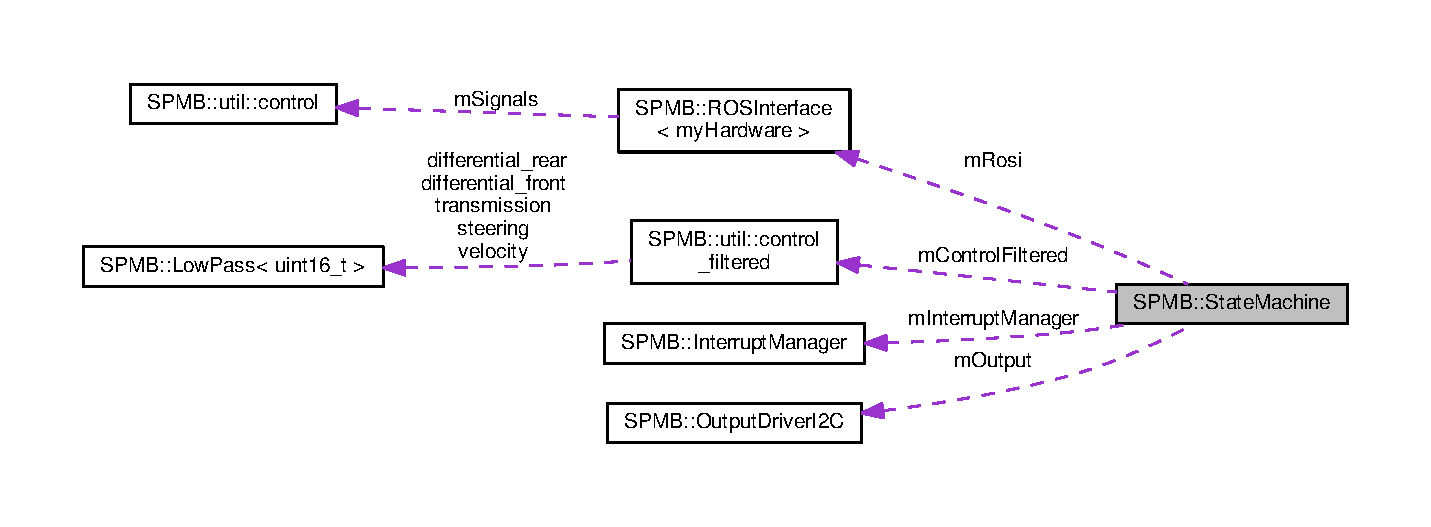
\includegraphics[width=350pt]{classSPMB_1_1StateMachine__coll__graph}
\end{center}
\end{figure}
\subsection*{Public Member Functions}
\begin{DoxyCompactItemize}
\item 
void \hyperlink{classSPMB_1_1StateMachine_a435a2eb92508aa038a0df64b4edd3ff2}{configure\+\_\+input} (\hyperlink{classSPMB_1_1InterruptManager}{Interrupt\+Manager} $\ast$interrupt\+\_\+manager\+\_\+in, \hyperlink{classSPMB_1_1ROSInterface}{R\+O\+S\+Interface}$<$ my\+Hardware $>$ $\ast$ros\+\_\+interface\+\_\+in)
\item 
void \hyperlink{classSPMB_1_1StateMachine_a1e1f84c67c0db8422a17c6d0f76f70a8}{configure\+\_\+output} (\hyperlink{classSPMB_1_1OutputDriverI2C}{Output\+Driver\+I2C} $\ast$output\+\_\+in)
\item 
void \hyperlink{classSPMB_1_1StateMachine_af1812d19f20f020a1635a96da3e8e048}{\+\_\+update\+\_\+rc\+\_\+signals} (\hyperlink{structSPMB_1_1util_1_1control}{util\+::control} \&signals\+\_\+rc)
\item 
void \hyperlink{classSPMB_1_1StateMachine_a1c01752d1ec267a1dc85924d453db6ce}{\+\_\+swl\+\_\+execute\+\_\+switching\+\_\+logic} (\hyperlink{structSPMB_1_1util_1_1control}{util\+::control} $\ast$signals\+\_\+rc)
\item 
void \hyperlink{classSPMB_1_1StateMachine_aefec64633728ccc393ff10752fe76243}{\+\_\+swl\+\_\+check\+\_\+idle\+\_\+transition} ()
\item 
void \hyperlink{classSPMB_1_1StateMachine_ad5b8e99beb2d19a29491429c45249179}{wait\+\_\+for\+\_\+next\+\_\+cycle} ()
\item 
void \hyperlink{classSPMB_1_1StateMachine_a8e7447f352e2a9b3f8d451bc834faaa2}{critical\+\_\+error} ()
\item 
void \hyperlink{classSPMB_1_1StateMachine_a46daaffbfb6385c230685dcba703314f}{\+\_\+process\+\_\+rc\+\_\+inputs} (\hyperlink{structSPMB_1_1util_1_1control}{util\+::control} \&signals\+\_\+rc)
\item 
void \hyperlink{classSPMB_1_1StateMachine_a6ffc09455280e241a558f1b46441aa9d}{\+\_\+process\+\_\+ros\+\_\+inputs} (\hyperlink{structSPMB_1_1util_1_1control}{util\+::control} \&signals\+\_\+ros)
\item 
void \hyperlink{classSPMB_1_1StateMachine_a651fcd0d71e1ce2ec7dfc72255ff8af7}{update\+\_\+output\+\_\+signals} ()
\item 
void \hyperlink{classSPMB_1_1StateMachine_a887475df9c15df2defce01f36030f931}{\+\_\+expose\+\_\+actuated\+\_\+signals\+\_\+to\+\_\+ros} ()
\item 
void \hyperlink{classSPMB_1_1StateMachine_a46d01bf4a019982fee4188d7434e38fa}{actuate} ()
\end{DoxyCompactItemize}
\subsection*{Public Attributes}
\begin{DoxyCompactItemize}
\item 
\hyperlink{classSPMB_1_1InterruptManager}{Interrupt\+Manager} $\ast$ \hyperlink{classSPMB_1_1StateMachine_a3e5c36f8ceb94e6f8913e7475cce2c40}{m\+Interrupt\+Manager}\hypertarget{classSPMB_1_1StateMachine_a3e5c36f8ceb94e6f8913e7475cce2c40}{}\label{classSPMB_1_1StateMachine_a3e5c36f8ceb94e6f8913e7475cce2c40}

\begin{DoxyCompactList}\small\item\em Pointer to interrupt manager provides access to all interrupt results. \end{DoxyCompactList}\item 
\hyperlink{classSPMB_1_1ROSInterface}{R\+O\+S\+Interface}$<$ my\+Hardware $>$ $\ast$ \hyperlink{classSPMB_1_1StateMachine_ab653add6890a51701f9d3a3760008e15}{m\+Rosi}\hypertarget{classSPMB_1_1StateMachine_ab653add6890a51701f9d3a3760008e15}{}\label{classSPMB_1_1StateMachine_ab653add6890a51701f9d3a3760008e15}

\begin{DoxyCompactList}\small\item\em Pointer to R\+OS interface that provides access to all R\+OS related actions. \end{DoxyCompactList}\item 
\hyperlink{classSPMB_1_1OutputDriverI2C}{Output\+Driver\+I2C} $\ast$ \hyperlink{classSPMB_1_1StateMachine_aecac5b27c3a5daa5331d367f55bed915}{m\+Output}\hypertarget{classSPMB_1_1StateMachine_aecac5b27c3a5daa5331d367f55bed915}{}\label{classSPMB_1_1StateMachine_aecac5b27c3a5daa5331d367f55bed915}

\begin{DoxyCompactList}\small\item\em Pointer to output driver that provides access to all hardware related actuation actions. \end{DoxyCompactList}\item 
\hyperlink{structSPMB_1_1util_1_1control__filtered}{util\+::control\+\_\+filtered} \hyperlink{classSPMB_1_1StateMachine_ac073bedbf77604e5df582b14e2a610cb}{m\+Control\+Filtered}\hypertarget{classSPMB_1_1StateMachine_ac073bedbf77604e5df582b14e2a610cb}{}\label{classSPMB_1_1StateMachine_ac073bedbf77604e5df582b14e2a610cb}

\begin{DoxyCompactList}\small\item\em Filtered control output for actuation via output driver. \end{DoxyCompactList}\item 
bool \hyperlink{classSPMB_1_1StateMachine_a856ca0d82b6c3da4d60c1a52d6982faf}{m\+A\+L\+I\+VE}\hypertarget{classSPMB_1_1StateMachine_a856ca0d82b6c3da4d60c1a52d6982faf}{}\label{classSPMB_1_1StateMachine_a856ca0d82b6c3da4d60c1a52d6982faf}

\begin{DoxyCompactList}\small\item\em Indicates state machine health status. \end{DoxyCompactList}\item 
bool \hyperlink{classSPMB_1_1StateMachine_ac0318161d8396b4190dfc57f2d7ca3e5}{m\+S\+W\+\_\+\+C\+O\+N\+T\+R\+O\+L\+\_\+\+A\+C\+T\+I\+VE}\hypertarget{classSPMB_1_1StateMachine_ac0318161d8396b4190dfc57f2d7ca3e5}{}\label{classSPMB_1_1StateMachine_ac0318161d8396b4190dfc57f2d7ca3e5}

\begin{DoxyCompactList}\small\item\em Activation boolean for software control loop. \end{DoxyCompactList}\item 
long \hyperlink{classSPMB_1_1StateMachine_a372848ebc671d9a34982345bc90a255d}{m\+S\+M\+Timestamp}\hypertarget{classSPMB_1_1StateMachine_a372848ebc671d9a34982345bc90a255d}{}\label{classSPMB_1_1StateMachine_a372848ebc671d9a34982345bc90a255d}

\begin{DoxyCompactList}\small\item\em Timestamp of last main loop iteration. \end{DoxyCompactList}\item 
long \hyperlink{classSPMB_1_1StateMachine_ab8b439f683f473ae15201e3928a279b1}{m\+C\+T\+R\+L\+Timestamp}\hypertarget{classSPMB_1_1StateMachine_ab8b439f683f473ae15201e3928a279b1}{}\label{classSPMB_1_1StateMachine_ab8b439f683f473ae15201e3928a279b1}

\begin{DoxyCompactList}\small\item\em Timestamp of last control actuation. \end{DoxyCompactList}\item 
uint16\+\_\+t \hyperlink{classSPMB_1_1StateMachine_af09b596c6c80e052807b56779d14903d}{m\+S\+M\+Time\+Period}\hypertarget{classSPMB_1_1StateMachine_af09b596c6c80e052807b56779d14903d}{}\label{classSPMB_1_1StateMachine_af09b596c6c80e052807b56779d14903d}

\begin{DoxyCompactList}\small\item\em Time period of main logic loop. \end{DoxyCompactList}\item 
uint16\+\_\+t \hyperlink{classSPMB_1_1StateMachine_a57244a6945d6a7442f67563dea8f1754}{m\+C\+T\+R\+L\+Time\+Period}\hypertarget{classSPMB_1_1StateMachine_a57244a6945d6a7442f67563dea8f1754}{}\label{classSPMB_1_1StateMachine_a57244a6945d6a7442f67563dea8f1754}

\begin{DoxyCompactList}\small\item\em Timp period of control loop. \end{DoxyCompactList}\item 
uint8\+\_\+t \hyperlink{classSPMB_1_1StateMachine_a4ef617b6025ddafc0c3d033cb59935d7}{m\+S\+W\+L\+State}\hypertarget{classSPMB_1_1StateMachine_a4ef617b6025ddafc0c3d033cb59935d7}{}\label{classSPMB_1_1StateMachine_a4ef617b6025ddafc0c3d033cb59935d7}

\begin{DoxyCompactList}\small\item\em State of switching logic, see macros for states. \end{DoxyCompactList}\item 
uint16\+\_\+t \hyperlink{classSPMB_1_1StateMachine_a9736947bcb2c289d85c7588434fb93c8}{m\+S\+W\+L\+Time\+Period}\hypertarget{classSPMB_1_1StateMachine_a9736947bcb2c289d85c7588434fb93c8}{}\label{classSPMB_1_1StateMachine_a9736947bcb2c289d85c7588434fb93c8}

\begin{DoxyCompactList}\small\item\em Time period of switching logic to detect idle. \end{DoxyCompactList}\item 
long \hyperlink{classSPMB_1_1StateMachine_acd7bdae2efc3414abcf4e0eba1b3ac59}{m\+S\+W\+L\+Timestamp}\hypertarget{classSPMB_1_1StateMachine_acd7bdae2efc3414abcf4e0eba1b3ac59}{}\label{classSPMB_1_1StateMachine_acd7bdae2efc3414abcf4e0eba1b3ac59}

\begin{DoxyCompactList}\small\item\em Timestamp of switching logic. \end{DoxyCompactList}\item 
boolean \hyperlink{classSPMB_1_1StateMachine_af37ba6ce3ef9826cd025a6259c42449d}{m\+S1}\hypertarget{classSPMB_1_1StateMachine_af37ba6ce3ef9826cd025a6259c42449d}{}\label{classSPMB_1_1StateMachine_af37ba6ce3ef9826cd025a6259c42449d}

\begin{DoxyCompactList}\small\item\em Channel 4 (differential\+\_\+front) state. \end{DoxyCompactList}\item 
boolean \hyperlink{classSPMB_1_1StateMachine_af7fcd1aec80eb5b7397b163db2e7c2ed}{m\+S2}\hypertarget{classSPMB_1_1StateMachine_af7fcd1aec80eb5b7397b163db2e7c2ed}{}\label{classSPMB_1_1StateMachine_af7fcd1aec80eb5b7397b163db2e7c2ed}

\begin{DoxyCompactList}\small\item\em Channel 5 (differential\+\_\+rear) state. \end{DoxyCompactList}\item 
boolean \hyperlink{classSPMB_1_1StateMachine_af6ffc5aa94ef7f423d217f8fba9cb998}{m\+S1\+\_\+prev}\hypertarget{classSPMB_1_1StateMachine_af6ffc5aa94ef7f423d217f8fba9cb998}{}\label{classSPMB_1_1StateMachine_af6ffc5aa94ef7f423d217f8fba9cb998}

\begin{DoxyCompactList}\small\item\em Previous Channel 4 (differential\+\_\+front) state. \end{DoxyCompactList}\item 
boolean \hyperlink{classSPMB_1_1StateMachine_a1d0a5cbe9d61f50e3d0ac3bdca99b936}{m\+S2\+\_\+prev}\hypertarget{classSPMB_1_1StateMachine_a1d0a5cbe9d61f50e3d0ac3bdca99b936}{}\label{classSPMB_1_1StateMachine_a1d0a5cbe9d61f50e3d0ac3bdca99b936}

\begin{DoxyCompactList}\small\item\em Previous Channel 5 (differential\+\_\+rear) state. \end{DoxyCompactList}\end{DoxyCompactItemize}


\subsection{Detailed Description}
A test class

\begin{DoxyRefDesc}{Todo}
\item[\hyperlink{todo__todo000001}{Todo}]Add status L\+ED class \end{DoxyRefDesc}


Definition at line 13 of file sm.\+h.



\subsection{Member Function Documentation}
\index{S\+P\+M\+B\+::\+State\+Machine@{S\+P\+M\+B\+::\+State\+Machine}!\+\_\+expose\+\_\+actuated\+\_\+signals\+\_\+to\+\_\+ros@{\+\_\+expose\+\_\+actuated\+\_\+signals\+\_\+to\+\_\+ros}}
\index{\+\_\+expose\+\_\+actuated\+\_\+signals\+\_\+to\+\_\+ros@{\+\_\+expose\+\_\+actuated\+\_\+signals\+\_\+to\+\_\+ros}!S\+P\+M\+B\+::\+State\+Machine@{S\+P\+M\+B\+::\+State\+Machine}}
\subsubsection[{\texorpdfstring{\+\_\+expose\+\_\+actuated\+\_\+signals\+\_\+to\+\_\+ros()}{_expose_actuated_signals_to_ros()}}]{\setlength{\rightskip}{0pt plus 5cm}void S\+P\+M\+B\+::\+State\+Machine\+::\+\_\+expose\+\_\+actuated\+\_\+signals\+\_\+to\+\_\+ros (
\begin{DoxyParamCaption}
{}
\end{DoxyParamCaption}
)}\hypertarget{classSPMB_1_1StateMachine_a887475df9c15df2defce01f36030f931}{}\label{classSPMB_1_1StateMachine_a887475df9c15df2defce01f36030f931}
expose ros 

Definition at line 217 of file sm.\+cpp.

\index{S\+P\+M\+B\+::\+State\+Machine@{S\+P\+M\+B\+::\+State\+Machine}!\+\_\+process\+\_\+rc\+\_\+inputs@{\+\_\+process\+\_\+rc\+\_\+inputs}}
\index{\+\_\+process\+\_\+rc\+\_\+inputs@{\+\_\+process\+\_\+rc\+\_\+inputs}!S\+P\+M\+B\+::\+State\+Machine@{S\+P\+M\+B\+::\+State\+Machine}}
\subsubsection[{\texorpdfstring{\+\_\+process\+\_\+rc\+\_\+inputs(util\+::control \&signals\+\_\+rc)}{_process_rc_inputs(util::control &signals_rc)}}]{\setlength{\rightskip}{0pt plus 5cm}void S\+P\+M\+B\+::\+State\+Machine\+::\+\_\+process\+\_\+rc\+\_\+inputs (
\begin{DoxyParamCaption}
\item[{{\bf util\+::control} \&}]{signals\+\_\+rc}
\end{DoxyParamCaption}
)}\hypertarget{classSPMB_1_1StateMachine_a46daaffbfb6385c230685dcba703314f}{}\label{classSPMB_1_1StateMachine_a46daaffbfb6385c230685dcba703314f}
taestestetest 

Definition at line 169 of file sm.\+cpp.

\index{S\+P\+M\+B\+::\+State\+Machine@{S\+P\+M\+B\+::\+State\+Machine}!\+\_\+process\+\_\+ros\+\_\+inputs@{\+\_\+process\+\_\+ros\+\_\+inputs}}
\index{\+\_\+process\+\_\+ros\+\_\+inputs@{\+\_\+process\+\_\+ros\+\_\+inputs}!S\+P\+M\+B\+::\+State\+Machine@{S\+P\+M\+B\+::\+State\+Machine}}
\subsubsection[{\texorpdfstring{\+\_\+process\+\_\+ros\+\_\+inputs(util\+::control \&signals\+\_\+ros)}{_process_ros_inputs(util::control &signals_ros)}}]{\setlength{\rightskip}{0pt plus 5cm}void S\+P\+M\+B\+::\+State\+Machine\+::\+\_\+process\+\_\+ros\+\_\+inputs (
\begin{DoxyParamCaption}
\item[{{\bf util\+::control} \&}]{signals\+\_\+ros}
\end{DoxyParamCaption}
)}\hypertarget{classSPMB_1_1StateMachine_a6ffc09455280e241a558f1b46441aa9d}{}\label{classSPMB_1_1StateMachine_a6ffc09455280e241a558f1b46441aa9d}
test ros 

Definition at line 175 of file sm.\+cpp.

\index{S\+P\+M\+B\+::\+State\+Machine@{S\+P\+M\+B\+::\+State\+Machine}!\+\_\+swl\+\_\+check\+\_\+idle\+\_\+transition@{\+\_\+swl\+\_\+check\+\_\+idle\+\_\+transition}}
\index{\+\_\+swl\+\_\+check\+\_\+idle\+\_\+transition@{\+\_\+swl\+\_\+check\+\_\+idle\+\_\+transition}!S\+P\+M\+B\+::\+State\+Machine@{S\+P\+M\+B\+::\+State\+Machine}}
\subsubsection[{\texorpdfstring{\+\_\+swl\+\_\+check\+\_\+idle\+\_\+transition()}{_swl_check_idle_transition()}}]{\setlength{\rightskip}{0pt plus 5cm}void S\+P\+M\+B\+::\+State\+Machine\+::\+\_\+swl\+\_\+check\+\_\+idle\+\_\+transition (
\begin{DoxyParamCaption}
{}
\end{DoxyParamCaption}
)}\hypertarget{classSPMB_1_1StateMachine_aefec64633728ccc393ff10752fe76243}{}\label{classSPMB_1_1StateMachine_aefec64633728ccc393ff10752fe76243}
oeoauu 

Definition at line 150 of file sm.\+cpp.

\index{S\+P\+M\+B\+::\+State\+Machine@{S\+P\+M\+B\+::\+State\+Machine}!\+\_\+swl\+\_\+execute\+\_\+switching\+\_\+logic@{\+\_\+swl\+\_\+execute\+\_\+switching\+\_\+logic}}
\index{\+\_\+swl\+\_\+execute\+\_\+switching\+\_\+logic@{\+\_\+swl\+\_\+execute\+\_\+switching\+\_\+logic}!S\+P\+M\+B\+::\+State\+Machine@{S\+P\+M\+B\+::\+State\+Machine}}
\subsubsection[{\texorpdfstring{\+\_\+swl\+\_\+execute\+\_\+switching\+\_\+logic(util\+::control $\ast$signals\+\_\+rc)}{_swl_execute_switching_logic(util::control *signals_rc)}}]{\setlength{\rightskip}{0pt plus 5cm}void S\+P\+M\+B\+::\+State\+Machine\+::\+\_\+swl\+\_\+execute\+\_\+switching\+\_\+logic (
\begin{DoxyParamCaption}
\item[{{\bf util\+::control} $\ast$}]{signals\+\_\+rc}
\end{DoxyParamCaption}
)}\hypertarget{classSPMB_1_1StateMachine_a1c01752d1ec267a1dc85924d453db6ce}{}\label{classSPMB_1_1StateMachine_a1c01752d1ec267a1dc85924d453db6ce}
taehu 

Definition at line 77 of file sm.\+cpp.

\index{S\+P\+M\+B\+::\+State\+Machine@{S\+P\+M\+B\+::\+State\+Machine}!\+\_\+update\+\_\+rc\+\_\+signals@{\+\_\+update\+\_\+rc\+\_\+signals}}
\index{\+\_\+update\+\_\+rc\+\_\+signals@{\+\_\+update\+\_\+rc\+\_\+signals}!S\+P\+M\+B\+::\+State\+Machine@{S\+P\+M\+B\+::\+State\+Machine}}
\subsubsection[{\texorpdfstring{\+\_\+update\+\_\+rc\+\_\+signals(util\+::control \&signals\+\_\+rc)}{_update_rc_signals(util::control &signals_rc)}}]{\setlength{\rightskip}{0pt plus 5cm}void S\+P\+M\+B\+::\+State\+Machine\+::\+\_\+update\+\_\+rc\+\_\+signals (
\begin{DoxyParamCaption}
\item[{{\bf util\+::control} \&}]{signals\+\_\+rc}
\end{DoxyParamCaption}
)}\hypertarget{classSPMB_1_1StateMachine_af1812d19f20f020a1635a96da3e8e048}{}\label{classSPMB_1_1StateMachine_af1812d19f20f020a1635a96da3e8e048}
update rc signals 

Definition at line 61 of file sm.\+cpp.

\index{S\+P\+M\+B\+::\+State\+Machine@{S\+P\+M\+B\+::\+State\+Machine}!actuate@{actuate}}
\index{actuate@{actuate}!S\+P\+M\+B\+::\+State\+Machine@{S\+P\+M\+B\+::\+State\+Machine}}
\subsubsection[{\texorpdfstring{actuate()}{actuate()}}]{\setlength{\rightskip}{0pt plus 5cm}void S\+P\+M\+B\+::\+State\+Machine\+::actuate (
\begin{DoxyParamCaption}
{}
\end{DoxyParamCaption}
)}\hypertarget{classSPMB_1_1StateMachine_a46d01bf4a019982fee4188d7434e38fa}{}\label{classSPMB_1_1StateMachine_a46d01bf4a019982fee4188d7434e38fa}
actuate 

Definition at line 224 of file sm.\+cpp.

\index{S\+P\+M\+B\+::\+State\+Machine@{S\+P\+M\+B\+::\+State\+Machine}!configure\+\_\+input@{configure\+\_\+input}}
\index{configure\+\_\+input@{configure\+\_\+input}!S\+P\+M\+B\+::\+State\+Machine@{S\+P\+M\+B\+::\+State\+Machine}}
\subsubsection[{\texorpdfstring{configure\+\_\+input(\+Interrupt\+Manager $\ast$interrupt\+\_\+manager\+\_\+in, R\+O\+S\+Interface$<$ my\+Hardware $>$ $\ast$ros\+\_\+interface\+\_\+in)}{configure_input(InterruptManager *interrupt_manager_in, ROSInterface< myHardware > *ros_interface_in)}}]{\setlength{\rightskip}{0pt plus 5cm}void S\+P\+M\+B\+::\+State\+Machine\+::configure\+\_\+input (
\begin{DoxyParamCaption}
\item[{{\bf Interrupt\+Manager} $\ast$}]{interrupt\+\_\+manager\+\_\+in, }
\item[{{\bf R\+O\+S\+Interface}$<$ my\+Hardware $>$ $\ast$}]{ros\+\_\+interface\+\_\+in}
\end{DoxyParamCaption}
)}\hypertarget{classSPMB_1_1StateMachine_a435a2eb92508aa038a0df64b4edd3ff2}{}\label{classSPMB_1_1StateMachine_a435a2eb92508aa038a0df64b4edd3ff2}
configure input 

Definition at line 25 of file sm.\+cpp.

\index{S\+P\+M\+B\+::\+State\+Machine@{S\+P\+M\+B\+::\+State\+Machine}!configure\+\_\+output@{configure\+\_\+output}}
\index{configure\+\_\+output@{configure\+\_\+output}!S\+P\+M\+B\+::\+State\+Machine@{S\+P\+M\+B\+::\+State\+Machine}}
\subsubsection[{\texorpdfstring{configure\+\_\+output(\+Output\+Driver\+I2\+C $\ast$output\+\_\+in)}{configure_output(OutputDriverI2C *output_in)}}]{\setlength{\rightskip}{0pt plus 5cm}void S\+P\+M\+B\+::\+State\+Machine\+::configure\+\_\+output (
\begin{DoxyParamCaption}
\item[{{\bf Output\+Driver\+I2C} $\ast$}]{output\+\_\+in}
\end{DoxyParamCaption}
)}\hypertarget{classSPMB_1_1StateMachine_a1e1f84c67c0db8422a17c6d0f76f70a8}{}\label{classSPMB_1_1StateMachine_a1e1f84c67c0db8422a17c6d0f76f70a8}
Brief description 

Definition at line 35 of file sm.\+cpp.

\index{S\+P\+M\+B\+::\+State\+Machine@{S\+P\+M\+B\+::\+State\+Machine}!critical\+\_\+error@{critical\+\_\+error}}
\index{critical\+\_\+error@{critical\+\_\+error}!S\+P\+M\+B\+::\+State\+Machine@{S\+P\+M\+B\+::\+State\+Machine}}
\subsubsection[{\texorpdfstring{critical\+\_\+error()}{critical_error()}}]{\setlength{\rightskip}{0pt plus 5cm}void S\+P\+M\+B\+::\+State\+Machine\+::critical\+\_\+error (
\begin{DoxyParamCaption}
{}
\end{DoxyParamCaption}
)}\hypertarget{classSPMB_1_1StateMachine_a8e7447f352e2a9b3f8d451bc834faaa2}{}\label{classSPMB_1_1StateMachine_a8e7447f352e2a9b3f8d451bc834faaa2}
thaeu 

Definition at line 57 of file sm.\+cpp.

\index{S\+P\+M\+B\+::\+State\+Machine@{S\+P\+M\+B\+::\+State\+Machine}!update\+\_\+output\+\_\+signals@{update\+\_\+output\+\_\+signals}}
\index{update\+\_\+output\+\_\+signals@{update\+\_\+output\+\_\+signals}!S\+P\+M\+B\+::\+State\+Machine@{S\+P\+M\+B\+::\+State\+Machine}}
\subsubsection[{\texorpdfstring{update\+\_\+output\+\_\+signals()}{update_output_signals()}}]{\setlength{\rightskip}{0pt plus 5cm}void S\+P\+M\+B\+::\+State\+Machine\+::update\+\_\+output\+\_\+signals (
\begin{DoxyParamCaption}
{}
\end{DoxyParamCaption}
)}\hypertarget{classSPMB_1_1StateMachine_a651fcd0d71e1ce2ec7dfc72255ff8af7}{}\label{classSPMB_1_1StateMachine_a651fcd0d71e1ce2ec7dfc72255ff8af7}
update output 

Definition at line 183 of file sm.\+cpp.

\index{S\+P\+M\+B\+::\+State\+Machine@{S\+P\+M\+B\+::\+State\+Machine}!wait\+\_\+for\+\_\+next\+\_\+cycle@{wait\+\_\+for\+\_\+next\+\_\+cycle}}
\index{wait\+\_\+for\+\_\+next\+\_\+cycle@{wait\+\_\+for\+\_\+next\+\_\+cycle}!S\+P\+M\+B\+::\+State\+Machine@{S\+P\+M\+B\+::\+State\+Machine}}
\subsubsection[{\texorpdfstring{wait\+\_\+for\+\_\+next\+\_\+cycle()}{wait_for_next_cycle()}}]{\setlength{\rightskip}{0pt plus 5cm}void S\+P\+M\+B\+::\+State\+Machine\+::wait\+\_\+for\+\_\+next\+\_\+cycle (
\begin{DoxyParamCaption}
{}
\end{DoxyParamCaption}
)}\hypertarget{classSPMB_1_1StateMachine_ad5b8e99beb2d19a29491429c45249179}{}\label{classSPMB_1_1StateMachine_ad5b8e99beb2d19a29491429c45249179}
oeauoeu 

Definition at line 39 of file sm.\+cpp.


\hypertarget{structSPMB_1_1util_1_1status__led}{}\section{S\+P\+MB\+:\+:util\+:\+:status\+\_\+led Struct Reference}
\label{structSPMB_1_1util_1_1status__led}\index{S\+P\+M\+B\+::util\+::status\+\_\+led@{S\+P\+M\+B\+::util\+::status\+\_\+led}}
\subsection*{Public Attributes}
\begin{DoxyCompactItemize}
\item 
uint8\+\_\+t {\bfseries off}\hypertarget{structSPMB_1_1util_1_1status__led_a6662fee00d36e8d23af9b00698b8193d}{}\label{structSPMB_1_1util_1_1status__led_a6662fee00d36e8d23af9b00698b8193d}

\item 
uint8\+\_\+t {\bfseries idle}\hypertarget{structSPMB_1_1util_1_1status__led_a9d7721d4c0c9948dce7df3415fdf836c}{}\label{structSPMB_1_1util_1_1status__led_a9d7721d4c0c9948dce7df3415fdf836c}

\item 
uint8\+\_\+t {\bfseries sw\+\_\+active}\hypertarget{structSPMB_1_1util_1_1status__led_a647beef9900026e1e516d456a111d5ad}{}\label{structSPMB_1_1util_1_1status__led_a647beef9900026e1e516d456a111d5ad}

\item 
uint8\+\_\+t {\bfseries rc\+\_\+intervention}\hypertarget{structSPMB_1_1util_1_1status__led_a1406160f915db22880b02941cbbc49fb}{}\label{structSPMB_1_1util_1_1status__led_a1406160f915db22880b02941cbbc49fb}

\end{DoxyCompactItemize}


\subsection{Detailed Description}


Definition at line 9 of file util.\+h.


%--- End generated contents ---

% Index
\backmatter
\newpage
\phantomsection
\clearemptydoublepage
\addcontentsline{toc}{chapter}{Index}
\printindex

\end{document}
